% RAVI (Reverse Action from Video): Learning Reverse Actions from Video -- JCSE (KIISE) regular paper draft.
% Build: pdflatex ravi; bibtex ravi; pdflatex ravi; pdflatex ravi
\documentclass{jcse}

\usepackage{url}
\usepackage{amsmath}
\usepackage{amssymb}
\usepackage{graphicx}
\usepackage{booktabs}
\usepackage{multirow}
\usepackage{tikz}
\usetikzlibrary{arrows.meta,positioning,fit,calc}
\definecolor{actc}{HTML}{2A78D6}  % agent / action
\definecolor{driftc}{HTML}{EB6834} % drift
\usepackage{algorithm}
\usepackage{algpseudocode}
\usepackage{flushend}
\papertype{Regular Paper}
\papertypeAtFoot{Open Access}
\volumeyear{Jan 0000} \volumenumber{00} \issuenumber{0} \pp{000-000}
\DOI{yy.5626/JCSE.2026.5.2.xxx}

\received{00 November 2026}
\revised{00 November 2026}
\accepted{00 November 2026}

\permissionUrl{http://jcse.kiise.org}

\copyrightString{Copyright \textcopyright 2026. The Korean Institute of Information Scientists and Engineers}

\issn{pISSN: 1976-4677 eISSN: 2093-8020}

\permission{
This is an Open Access article distributed under the terms of the Creative Commons Attribution Non-Commercial License (\url{http://creativecommons.org/licenses/
by-nc/3.0/}) which permits unrestricted non-commercial use, distribution, and reproduction in any medium, provided the original work is properly cited.
}


\newcommand{\method}{RAVI}
\newcommand{\zb}{\bar{z}}
\newcommand{\zundo}{z_{\mathrm{undo}}}
\newcommand{\R}{\mathbb{R}}
\newcommand{\sym}{\mathrm{sym}}
\newcommand{\cond}{\mathrm{cond}}
\newcommand{\zss}{z^{\mathrm{ss}}}
\newcommand{\klin}{\kappa^{\mathrm{lin}}}
% Revision 1: red markers flag results that need the new runs of code/run_all.sh (see REVISION_CHECKLIST.md).
\newcommand{\todo}[1]{\textcolor{red}{[TODO: #1]}}
\newcommand{\tbd}{\textcolor{red}{tbd}}

\title[Learning Reverse Actions from Video]{Learning Reverse Actions from Video}
\author{
	\authname{Patrick Mokodir Emaase} \\
	\affaddr{Department of Computer Science and Engineering, Seoul National University, Seoul, Korea}
	\email{emaase@bi.snu.ac.kr} \\
	\\
	\authname{Choi Suhyung} \\
	\affaddr{AI Institute, Seoul National University, Seoul, Korea}
	\email{shchoi@bi.snu.ac.kr} \\
	\\
	\authname{Byoung Tak Zhang$^*$} \\
	\affaddr{Department of Computer Science and Engineering, Seoul National University, Seoul, Korea}
	\email{btzhang@snu.ac.kr} \\
}
\shortauthors{P.M. Emaase, S. Choi and B.T. Zhang}
\bottomstuff{$^*$ Corresponding Author}
\category{Smart and Intelligent Computing}
\keywords{Latent action models; Koopman operator; reversibility; learning from video; robot manipulation; world models}

\begin{document}

\begin{abstract}
Latent action models learn controllable dynamics from action-free video, but only in forward time, although undoing mistakes, planning backward and judging reversibility all need the reverse direction.
A common shortcut to reversal is to require that a frame pair played backward be explained by the negated forward action.
We show that, for a latent action model of Koopman form, this is consistent only if the scene has no motion of its own, so that falling and settling must be attributed to the agent.
We introduce {\method} (Reverse Action from Video), where the latent action moves a lifted state through a Koopman operator and the scene's own motion is modelled by a drift generator distinct from the generators of the agent's actions.
Trained on forward footage only, {\method} yields closed-form expressions for the backward step, the time-reversal action of the first-order latent dynamics, the undo action and a per-step reversibility score; we establish when each one is exact, characterise single-step undo both for all states and for a single transition, and show that the score depends only on the inferred action.
On 100 real bimanual robot recordings in which bread is placed into a toaster or taken out of it, Koopman models with a drift generator keep reverse rollouts stable (end-distance ratio 0.74--0.84) where an MLP sign-reversal model diverges (1.55--1.86), but a plain latent action model without any reversal constraint is equally stable and flags irreversible drops equally well; {\method} adapts best to the opposite task, and a dropped object still cannot be restored in one step.
In a controlled study with known dissipative drift, decoding swapped pairs under the reversed drift absorbs less passive motion than sign reversal, but the reversibility score tracks motion rather than irreversibility, and a plain latent action model undoes reversible steps best.
\end{abstract}

\maketitle

% =====================================================================
\section{Introduction} \label{s:intro}

Learning to act from video is attractive because video is abundant and action labels are not.
Latent action models (LAMs) exploit this by inferring a latent action $z$ from a pair of consecutive frames $(o_t,o_{t+1})$ with an inverse dynamics model, and by training a forward model to predict $o_{t+1}$ from $o_t$ and $z$~\cite{schmidt2024lapo,bruce2024genie}.
The learned latent actions then serve as pseudo-labels for policy pretraining, so that large collections of unlabeled video can be turned into control knowledge~\cite{ye2025lapa}.

LAMs are trained only in forward time.
Many uses, however, need the reverse direction.
A robot that has made a mistake must undo it; a planner can search backward from a goal; an autonomous system must reset itself without human help; and a safe agent must judge whether an action can be reversed at all~\cite{grinsztajn2021reversibility,lai2020bmpo,goyal2019recall,eysenbach2018leave}.
To make reversal inexpensive, several recent models impose algebraic structure on their latent actions.
Examples are additive composition of latent actions~\cite{wei2026aclam}, a consistency term asking that a swapped frame pair be explained by the negated forward action~\cite{tang2026alam}, and group-action constraints imposed on world models~\cite{wang2026groupactions,keurti2023hae}.

All of them rest on one premise: reversing an action amounts to flipping its sign.
The premise is valid only if the scene has no motion of its own.
Physical scenes, however, contain \emph{drift}---gravity, friction, objects coming to rest, and other agents.
Once drift is present, two distinct notions of a ``backward action'' must be separated.
The \textbf{time-reversal action} accounts for the clip played backward, with the physics reversed as well; the \textbf{undo action} brings the scene back to its previous state while the ordinary physics keeps acting.
Consider a slice of bread released above a toaster slot: while the agent does nothing, it drops into the slot and comes to rest.
Played backward, it climbs out of the slot with no action at all, yet restoring it in reality requires the agent to reach in and lift it.
With one forward model shared by both orderings, a sign-reversal loss cannot accommodate both situations; it ends up attributing the drop to the agent.

Time reversal needs care here.
For a mechanical system whose state includes velocity, reversing time flips the velocities and leaves conservative forces such as gravity unchanged, so only dissipation---the impact and friction that bring the slice to rest---makes the reversed clip impossible.
Latent states computed from a single frame carry no velocity, and their dynamics are first order; for such states time reversal negates the whole drift, and this is the setting we study (Section~\ref{s:problem}).

We present {\method} (Reverse Action from Video), a latent action model in which the agent's contribution to the dynamics is kept apart from the scene's autonomous motion.
{\method} learns a lifted latent state on which a latent action acts through a Koopman operator~\cite{koopman1931,mezic2005spectral,brunton2022modern}
\begin{equation}
K(z)=\exp\Big(G_0+\sum_{i=1}^m z_iG_i\Big),
\label{e:koopman}
\end{equation}
with a drift generator $G_0$ that is kept separate from the action generators $G_i$.
The choice follows a standard property: for control-affine dynamics the Koopman generator depends affinely on the input~\cite{goswami2017global,bruder2021bilinear} (Proposition~\ref{p:affine}), and models of this form are well established for prediction and control~\cite{korda2018koopman,bruder2021bilinear}.
Since $z$ enters the generator linearly, all reverse quantities can be written down in closed form from a model fitted to forward footage.

\paragraph{Contributions.} This paper makes the following contributions.
\begin{enumerate}
	\item \textbf{Two reverse actions, defined and derived.} We give formal definitions of the time-reversal and undo actions for first-order latent dynamics and obtain both in closed form within {\method}: $\zb=-z$ with the drift negated, and $\zundo=-z-2c$, with $c$ the latent action that most closely imitates the drift on the states the robot visits.
	\item \textbf{Theory.} We show that each learned step has an exact inverse in the lifted space and that the time-reversal action requires no commutativity between generators, and we characterise when one step suffices to undo a transition, both from every state and, to first order, for a single transition. We further show that a Koopman sign-reversal model can be consistent only with zero drift and that the agent/drift split is not identifiable from action-free video. We bound the reversibility score by the symmetric part of the generator, show that it depends on the inferred action alone, and give a reference value for the drift residual when actions and drift are unrelated.
	\item \textbf{A drift-aware reversal loss} that decodes swapped frame pairs under the reversed drift $-G_0$. Given the exact inverse, it reduces to backward reconstruction plus antisymmetry of the inverse dynamics model (Remark~\ref{r:reduce}); a Koopman ablation that decodes the swapped pair under $+G_0$ instead tests whether the sign of the drift matters.
	\item \textbf{A real-robot evaluation} on 100 bimanual ALOHA episodes~\cite{zhao2023aloha} of inserting bread into a toaster and removing it, with 5-fold cross-validation in both transfer directions, fold-level paired statistics and null references, and a controlled study with known dissipative drift and ground-truth reversibility, supported in the appendices by per-fold results, development runs and a step-by-step walkthrough of every model variable.
\end{enumerate}

\paragraph{Findings.}
Koopman models with a drift generator keep reverse rollouts stable where an MLP sign-reversal model diverges, detect irreversible moments well above chance, and transfer best to the opposite task when only the inverse dynamics model is adapted.
The evaluation also marks clear limits: a plain LAM without any reversal constraint is equally stable, matches {\method} on reversibility detection and beats it on action alignment; the robot-idle anchor raises detection in every fold but slows transfer; the reversibility score depends only on the inferred action, so it cannot isolate passive motion by itself; and a dropped slice cannot be undone in one step.
A controlled study with known dissipative drift (Section~\ref{s:toy}) confirms that decoding under $-G_0$ absorbs less drift than under $+G_0$ and that the drift correction improves the undo action, but also shows that $\kappa_t$ tracks motion rather than irreversibility and that a plain LAM undoes reversible steps best.

The rest of the paper is organised as follows.
Section~\ref{s:related} reviews related work.
Section~\ref{s:problem} defines the problem, Section~\ref{s:method} presents {\method}, and Section~\ref{s:theory} gives its theory.
Section~\ref{s:setup} describes the experimental setup, Section~\ref{s:results} reports the results, Section~\ref{s:discussion} discusses limitations and Section~\ref{s:conclusion} concludes; the appendices give further results, a controlled study, development runs and implementation details.

% =====================================================================
\section{Related Work} \label{s:related}

\subsection{Latent Action Models}
LAPO~\cite{schmidt2024lapo} and Genie~\cite{bruce2024genie} learn latent actions from video by pairing an inverse dynamics model (IDM) with a forward model behind an information bottleneck, so that the latent action must explain the change between frames without copying the next frame.
LAPA~\cite{ye2025lapa} uses such latent actions to pretrain vision-language-action policies without robot action labels.
Zhang et al.~\cite{zhang2025lams} study what LAMs actually capture and find that changes not caused by the agent, background motion for instance, also enter the latent action unless augmentation or a handful of action labels are added.
Their finding already hints that LAMs blend the agent's effect with passive scene dynamics; we address the consequence of this blending for the reverse direction.

\subsection{Algebraic Structure in Latent Actions}
Several works impose group structure on latent actions.
The homomorphism autoencoder learns a group representation that acts linearly on the latent space~\cite{keurti2023hae}.
AC-LAM enforces additive composition of latent actions over short horizons~\cite{wei2026aclam}.
ALAM regularises continuous latents with a composition loss and a reversal loss that asks the action of a swapped pair to equal the negated forward action, and it lists irreversible dynamics among its limitations~\cite{tang2026alam}.
Wang et al. view action-conditioned world models as group actions and impose identity, inverse and composition consistency~\cite{wang2026groupactions}.
In each case an action and its inverse are assumed to act on a state space without drift.
{\method} keeps the inverse structure but separates drift from action, and shows why sign reversal in Koopman form fails when drift is present.

\subsection{Reversibility and Backward Models}
Backward models generate trajectories that lead to high-value states~\cite{goyal2019recall} or are combined with forward models for policy optimisation~\cite{lai2020bmpo}.
Reversibility-aware reinforcement learning estimates whether an action can be undone from the temporal order of events~\cite{grinsztajn2021reversibility}, and reset-free learning trains a policy to undo the forward policy~\cite{eysenbach2018leave}.
The arrow of time can also be learned from video directly~\cite{wei2018arrow}.
These methods either assume known actions or do not provide a reverse action; {\method} derives reverse actions and a reversibility score from action-free video.

\subsection{Koopman Operators for Learning and Control}
The Koopman operator represents nonlinear dynamics as a linear operator on observables~\cite{koopman1931,mezic2005spectral}.
Data-driven approximations with learned observables~\cite{lusch2018deep} and their extensions to control~\cite{korda2018koopman,bruder2021bilinear,brunton2022modern} are widely used for prediction and model predictive control, including for soft robots~\cite{bruder2019soft}.
Dynamic mode decomposition with control fits linear models with an additive input term~\cite{proctor2016dmdc}, and for control-affine systems the Koopman generator is affine in the input, which yields bilinear lifted models~\cite{goswami2017global,bruder2021bilinear}.
{\method} uses this structure for a different purpose: the separation of drift and input terms in the generator defines reverse actions, and the spectrum of the step operator yields a reversibility score.

\subsection{Deformable Object Manipulation}
Cloth manipulation combines quasi-static and dynamic motions~\cite{lin2020softgym,lin2021vcd}; unfolding often relies on flings or regrasps rather than replaying folds~\cite{ha2021flingbot,avigal2022speedfolding}.
We return to this setting as future work in Section~\ref{s:discussion}.

% =====================================================================
\section{Problem Formulation} \label{s:problem}

We observe videos $\{o_1,\dots,o_T\}$ of an agent acting in a scene, without action labels.
The scene evolves under the agent's unknown actions and under its own passive dynamics.
We model the latent dynamics as a control-affine system on a lifted state $s$,
\begin{equation}
\dot{s}=f(s)+\sum_{i=1}^m u_i\,g_i(s),
\label{e:cas}
\end{equation}
where $f$ is the drift and $g_i$ are the input vector fields.
A latent action $z\in\R^m$ summarises the input applied over one step of length $\Delta t$.
Eq.~(\ref{e:cas}) is first order in $s$; when $s$ is computed from a single frame, as in this paper, it carries no velocity, and inertial effects can be represented only approximately.

\begin{definition}[Time-reversal action]
\label{d:trev}
Given a forward transition $s_t\to s_{t+1}$ under action $z$, the time-reversal action $\zb$ is the action that reproduces the reversed transition $s_{t+1}\to s_t$ in the reversed world, in which the drift is negated and the input vector fields are unchanged.
\end{definition}

Definition~\ref{d:trev} is the time reversal of the first-order system~(\ref{e:cas}): if $s(t)$ solves~(\ref{e:cas}) under input $u(t)$, then $s(-t)$ solves it with $f$ replaced by $-f$ and input $-u(-t)$.
It agrees with physical time reversal only for dissipative and quasi-static motion.
For a second-order system with velocity in the state, physical time reversal flips the velocities and leaves conservative forces unchanged, so a freely falling object seen in reverse obeys ordinary gravity.
A frame-based latent state cannot express that distinction, and we therefore read Definition~\ref{d:trev} as a statement about the learned first-order dynamics rather than about the underlying mechanics.

\begin{definition}[Undo action]
\label{d:undo}
Given a forward transition $s_t\to s_{t+1}$ under action $z$, an undo action $\zundo$ is an action that returns the state from $s_{t+1}$ to $s_t$ under the real, forward-time dynamics, including the drift.
It is \emph{state-independent} if it undoes the step $z$ from every state, and \emph{state-specific} if it returns only this $s_{t+1}$ to $s_t$.
\end{definition}

The two actions coincide when $f=0$.
With drift they differ, and a model trained only in forward time must recover both.
Our goal is to learn, from forward videos alone, a model that (i) predicts forward and backward, (ii) yields both reverse actions in closed form, (iii) scores how reversible each step is, and (iv) transfers to the reverse task with little data.

% =====================================================================
\section{The {\method} Model} \label{s:method}

\begin{figure*}[t]
\centering
\resizebox{\textwidth}{!}{%
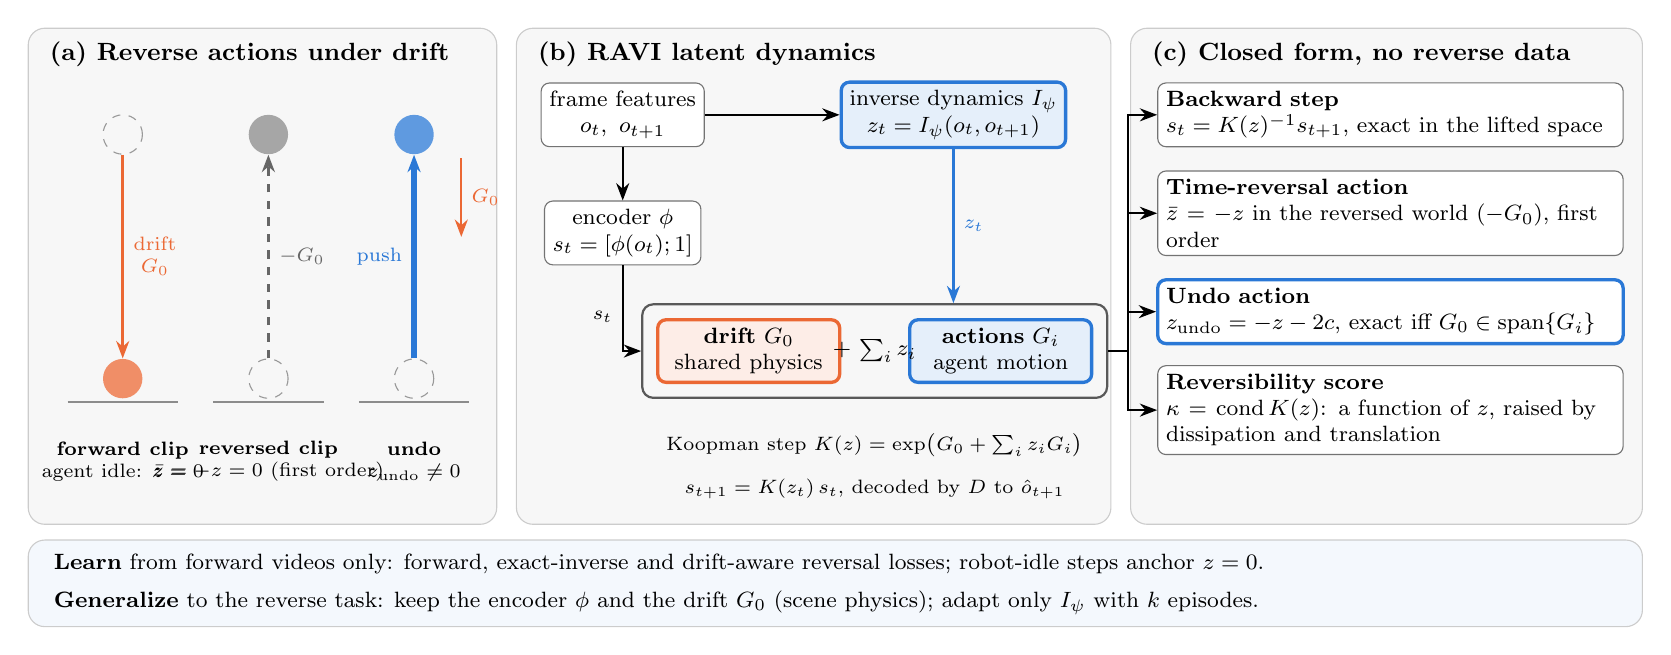
\begin{tikzpicture}[
	font=\footnotesize, >={Stealth[length=2.2mm]},
	box/.style={draw=black!55, rounded corners=3pt, align=center, inner sep=3pt, fill=white},
	driftbox/.style={box, draw=driftc, fill=driftc!12, very thick, text width=2.1cm},
	actbox/.style={box, draw=actc, fill=actc!12, very thick},
	outbox/.style={box, text width=5.7cm, align=left},
	panel/.style={draw=black!20, fill=black!3, rounded corners=6pt},
	ttl/.style={font=\small\bfseries, anchor=west},
	note/.style={font=\scriptsize, align=center},
	ball/.style={circle, minimum size=5mm, inner sep=0pt},
]
% ---------- panels
\draw[panel] (-0.2,0.75) rectangle (5.75,7.05);
\draw[panel] (6.0,0.75) rectangle (13.55,7.05);
\draw[panel] (13.8,0.75) rectangle (20.3,7.05);
\node[ttl] at (-0.05,6.72) {(a) Reverse actions under drift};
\node[ttl] at (6.15,6.72) {(b) RAVI latent dynamics};
\node[ttl] at (13.95,6.72) {(c) Closed form, no reverse data};

% ---------- (a) a falling object seen three ways
\foreach \x in {1.0,2.85,4.7} { \draw[black!45, thick] (\x-0.7,2.3) -- (\x+0.7,2.3); }
% forward clip: the object falls under drift while the agent is idle
\node[ball, draw=black!40, dashed] (f0) at (1.0,5.7) {};
\node[ball, fill=driftc!75] (f1) at (1.0,2.6) {};
\draw[->, driftc, very thick] (f0) -- node[right, note]{drift\\$G_0$} (f1);
\node[note] at (1.0,1.55) {\textbf{forward clip}\\agent idle: $z=0$};
% reversed clip: rises with zero action under reversed drift
\node[ball, draw=black!40, dashed] (r0) at (2.85,2.6) {};
\node[ball, fill=black!35] (r1) at (2.85,5.7) {};
\draw[->, black!60, very thick, dashed] (r0) -- node[right, note]{$-G_0$} (r1);
\node[note] at (2.85,1.55) {\textbf{reversed clip}\\$\bar z=-z=0$ (first order)};
% undo: the agent must push against the drift
\node[ball, draw=black!40, dashed] (u0) at (4.7,2.6) {};
\node[ball, fill=actc!75] (u1) at (4.7,5.7) {};
\draw[->, actc, line width=2pt] (u0) -- node[left, note]{push} (u1);
\draw[->, driftc, thick] (5.3,5.4) -- node[right, note]{$G_0$} (5.3,4.4);
\node[note] at (4.7,1.55) {\textbf{undo}\\$z_{\mathrm{undo}}\neq0$};

% ---------- (b) model
\node[box] (frames) at (7.35,5.95) {frame features\\$o_t,\ o_{t+1}$};
\node[box] (enc) at (7.35,4.45) {encoder $\phi$\\$s_t=[\phi(o_t);1]$};
\node[actbox] (idm) at (11.55,5.95) {inverse dynamics $I_\psi$\\$z_t=I_\psi(o_t,o_{t+1})$};
\node[driftbox] (g0) at (8.95,2.95) {\textbf{drift} $G_0$\\shared physics};
\node[actbox, text width=2.1cm] (gi) at (12.15,2.95) {\textbf{actions} $G_i$\\agent motion};
\node[font=\footnotesize] (plus) at (10.55,2.95) {$+\,\sum_i z_i$};
\node[draw=black!65, rounded corners=4pt, thick, fit=(g0)(gi)(plus), inner sep=5pt] (K) {};
\node[note] at (10.55,1.75) {Koopman step $K(z)=\exp\!\big(G_0+\sum_i z_iG_i\big)$};
\node[note] at (10.55,1.2) {$s_{t+1}=K(z_t)\,s_t$, decoded by $D$ to $\hat o_{t+1}$};
\draw[->, thick] (frames) -- (enc);
\draw[->, thick] (frames) -- (idm);
\draw[->, thick] (enc.south) |- node[pos=0.3, left, note]{$s_t$} (K.west);
\draw[->, thick, actc] (idm.south) -- node[right, note]{$z_t$} (idm.south |- K.north);

% ---------- (c) outputs
\node[outbox] (o1) at (17.1,5.95) {\textbf{Backward step}\\$s_t=K(z)^{-1}s_{t+1}$, exact in the lifted space};
\node[outbox] (o2) at (17.1,4.7) {\textbf{Time-reversal action}\\$\bar z=-z$ in the reversed world ($-G_0$), first order};
\node[outbox, draw=actc, very thick] (o3) at (17.1,3.45) {\textbf{Undo action}\\$z_{\mathrm{undo}}=-z-2c$, exact iff $G_0\in\mathrm{span}\{G_i\}$};
\node[outbox] (o4) at (17.1,2.2) {\textbf{Reversibility score}\\$\kappa=\mathrm{cond}\,K(z)$: a function of $z$, raised by dissipation and translation};
\coordinate (bus) at ($(K.east)+(0.25,0)$);
\draw[thick] (K.east) -- (bus);
\foreach \o in {o1,o2,o3,o4} { \draw[->, thick] (bus) |- (\o.west); }

% ---------- bottom strip: learning and generalization
\draw[panel, fill=actc!5] (-0.2,-0.55) rectangle (20.3,0.55);
\node[anchor=west] at (0.0,0.25) {\textbf{Learn} from forward videos only: forward, exact-inverse and drift-aware reversal losses; robot-idle steps anchor $z=0$.};
\node[anchor=west] at (0.0,-0.25) {\textbf{Generalize} to the reverse task: keep the encoder $\phi$ and the drift $G_0$ (scene physics); adapt only $I_\psi$ with $k$ episodes.};
\end{tikzpicture}}
\caption{RAVI at a glance. (a) Under drift there are two reverse actions: played backward, an object that dropped and came to rest climbs with no action, whereas restoring it in the real world requires a push against the drift. (b) RAVI lifts frames to a state $s_t$ and lets the latent action act through a Koopman operator whose drift generator $G_0$ (scene physics, shared across tasks) is separate from the action generators $G_i$ (agent motion). (c) Every reverse quantity follows in closed form from the forward model; the condition number $\kappa$ depends only on the inferred action and also grows with translations of the lifted state (Corollary~\ref{c:kappa}). The design is task-independent; the instantiation used in our experiments is shown in \ref{a:impl} (Fig.~\ref{f:pipeline}).}
\label{f:concept}
\end{figure*}

From forward footage, {\method} fits a single latent dynamics model and reads every reverse quantity off it (Fig.~\ref{f:concept}).
The key modelling choice is that a task and its reverse occupy the same scene states and obey the same passive physics, while the agent moves differently in each.
Loading bread into a toaster and unloading it, for example, pass through identical plate and slot configurations under identical gravity, but with different grasps and trajectories.
Accordingly, the encoder and the drift are common to both tasks, and only the latent actions are task specific.

\subsection{Lifted State and Latent Action}
Each frame is encoded by a frozen visual backbone and a trainable head $\phi$, and a constant coordinate is appended to form the lifted state,
\begin{equation}
s_t=[\phi(o_t);1]\in\R^{d+1},\qquad z_t=I_\psi(o_t,o_{t+1})\in\R^{m}.
\label{e:state}
\end{equation}
The constant coordinate makes translations linear and keeps the constant observable, which is always a Koopman eigenfunction with eigenvalue 1.
The IDM receives $[o_t,o_{t+1},o_{t+1}-o_t]$.
Here $o_t$ denotes the frozen backbone's features of frame $t$ (Section~\ref{s:setup}); the head, the IDM and the decoder all operate on these features, and we write $x_t=\phi(o_t)$ for the non-constant part of $s_t$.

\subsection{Drift-Aware Koopman Dynamics}
The latent action acts through Eq.~(\ref{e:koopman}), $s_{t+1}=K(z_t)\,s_t$.
We parameterise the generators as
\begin{align}
G_0&=\begin{bmatrix} S-S^\top-LL^\top & b_0\\ 0 & 0\end{bmatrix},\nonumber\\
G_i&=\begin{bmatrix} W_i-W_i^\top+\sym(V_i) & b_i\\ 0 & 0\end{bmatrix},
\label{e:gens}
\end{align}
with $\sym(V)=(V+V^\top)/2$.
The last row is zero, so the constant coordinate stays 1.
An action generator combines a skew-symmetric block, a weakly L2-penalised symmetric block and a translation column, which keeps pure actions close to rigid motions in the lifted space.
The drift has a skew part and a negative semidefinite part $-LL^\top$, which carries dissipation such as falling, friction and settling.
We write $M(z)$ for the upper-left $d\times d$ block of $A(z)=G_0+\sum_iz_iG_i$.

\subsection{Reverse Quantities}
\textbf{Backward step.} Since every step can be inverted exactly (Proposition~\ref{p:inverse}), the preceding state is recovered without additional parameters:
\begin{equation}
s_t=e^{-A(z_t)}\,s_{t+1},\qquad A(z_t)=G_0+\textstyle\sum_iz_{t,i}G_i.
\label{e:backward}
\end{equation}
Decoding still passes through $D$, so in feature space the backward step is as accurate as the forward model.

\textbf{Time-reversal action.} Reversing time negates the drift to $-G_0$ but leaves the action generators untouched, so $\zb=-z$ accounts for the reversed clip (Proposition~\ref{p:trev}), for the first-order latent dynamics of Definition~\ref{d:trev}.

\textbf{Undo action.} To undo the step from every state in a single step under the ordinary, forward-time dynamics, an action $z'$ must satisfy $G_0+\sum_iz'_iG_i=-(G_0+\sum_iz_iG_i)$, which leads to
\begin{align}
\zundo&=-z-2c,\nonumber\\
c&=\arg\min_c\ \mathbb{E}_{s\sim\mathcal{D}}\Big\|\Big(G_0-\sum_ic_iG_i\Big)s\Big\|^2,
\label{e:undo}
\end{align}
with $c$ the latent action whose effect on the visited states $\mathcal{D}$ is closest to that of the drift.
We fit $c$ on states and not on full matrices for a reason: $m=16$ generators cannot span all $65\times65$ matrices, yet they may still offset the drift in the region the robot actually visits.
For a single transition a weaker condition suffices, and we also compute a state-specific undo action
\begin{equation}
\zss_t=\arg\min_{z'}\big\|D\big(K(z')\,s_{t+1}\big)-o_t\big\|^2,
\label{e:undoss}
\end{equation}
a problem in $m=16$ unknowns that we solve by gradient descent from $-z_t-2c$; to first order in the lifted space it is a linear least-squares problem (Proposition~\ref{p:undo}(d)).
An $H$-step plan optimises $H$ actions jointly through the composed operator.
The normalised residual
\begin{equation}
\varepsilon=\frac{\big(\mathbb{E}_s\|(G_0-\sum_ic_iG_i)s\|^2\big)^{1/2}}{\big(\mathbb{E}_s\|G_0s\|^2\big)^{1/2}}
\label{e:residual}
\end{equation}
measures the part of the drift that no state-independent action can cancel; Proposition~\ref{p:undo} shows that it controls the error of the undo action to first order.
The per-transition residual $\varepsilon_t=\|(G_0-\sum_ic_iG_i)s_t\|/\|G_0s_t\|$ localises where the drift is not cancelled.
A residual near 1 must be read against Remark~\ref{r:eps}: unrelated actions and drift would also produce it.

\textbf{Reversibility score.} For each transition we report $\kappa_t=\cond(K(z_t))=\sigma_{\max}/\sigma_{\min}$.
Proposition~\ref{p:kappa} shows that $\kappa_t$ can exceed 1 only through the symmetric part of the generator, which in {\method} collects the dissipative drift, the symmetric action blocks and the translation columns.
Corollary~\ref{c:kappa} adds two qualifications: $\kappa_t$ depends on the transition only through $z_t$, and translations of the lifted state raise it.
We therefore also evaluate the translation-free score $\klin_t=\cond(e^{M(z_t)})$ and the state-dependent contraction rate of the drift, $\rho_t=\|L^\top x_t\|^2/\|x_t\|^2$.

\subsection{Anchoring the Agent/Drift Split} \label{s:anchor}
The change $z\to z+c$ with $G_0\to G_0-\sum_ic_iG_i$ leaves every forward prediction unchanged (Proposition~\ref{p:gauge}).
{\method} anchors this freedom with robot-idle steps $\mathcal{N}$, on which the agent is known not to act, by requiring $z_t\approx0$ there.
Idle steps are identified from proprioceptive joint speed.
No action labels are used, but joint speed is a non-visual signal, so the anchored model is not trained from video alone; {\method} without the anchor is.

\subsection{Training Objective}
With a decoder $D$ and the reversed latent action $\zb_t=I_\psi(o_{t+1},o_t)$, {\method} minimises
\begin{align}
\mathcal{L}&=\ell_{\mathrm{fwd}}+\lambda_b\,\ell_{\mathrm{bwd}}+\lambda_r\,(\ell_{\mathrm{rev}}+\ell_{\mathrm{neg}})\nonumber\\
&\quad+\lambda_a\,\ell_{\mathrm{idle}}+\lambda_v\,\Omega+\mathcal{L}_{\mathrm{rec}},\nonumber\\
\ell_{\mathrm{fwd}}&=\big\|o_{t+1}-D\big(e^{A(z_t)}s_t\big)\big\|^2,\nonumber\\
\ell_{\mathrm{bwd}}&=\big\|o_t-D\big(e^{-A(z_t)}s_{t+1}\big)\big\|^2,\nonumber\\
\ell_{\mathrm{rev}}&=\big\|o_t-D\big(e^{-G_0+\sum_i\zb_{t,i}G_i}s_{t+1}\big)\big\|^2,\nonumber\\
\ell_{\mathrm{neg}}&=\|z_t+\zb_t\|^2,\quad \ell_{\mathrm{idle}}=\textstyle\sum_{t\in\mathcal{N}}\|z_t\|^2,\nonumber\\
\Omega&=\textstyle\sum_i\|V_i\|_F^2,
\label{e:loss}
\end{align}
where $\mathcal{L}_{\mathrm{rec}}$ reconstructs $o_t$ and $o_{t+1}$ from their lifted states and also includes a latent consistency term $\|K(z_t)s_t-s_{t+1}\|^2$.
Together, $\ell_{\mathrm{rev}}$ and $\ell_{\mathrm{neg}}$ form the \emph{drift-aware reversal loss}, which decodes the swapped pair with the drift reversed to $-G_0$; sign-reversal losses~\cite{tang2026alam} instead keep the forward drift.
Proposition~\ref{p:signrev} shows why this distinction matters, and Remark~\ref{r:reduce} that, once $\zb_t=-z_t$, $\ell_{\mathrm{rev}}$ coincides with $\ell_{\mathrm{bwd}}$, so the practical role of the drift-aware loss is to make the IDM antisymmetric on swapped pairs.
Algorithm~\ref{a:wao} summarises training and the closed-form reverse quantities.

\begin{algorithm}[t]
\caption{{\method}: training on forward videos and closed-form reverse quantities}\label{a:wao}
\begin{algorithmic}[1]
\Require forward videos, idle set $\mathcal{N}$, weights $\lambda_b,\lambda_r,\lambda_a,\lambda_v$
\Repeat
	\State sample transitions $(o_t,o_{t+1})$ with idle flags
	\State $s_t\gets[\phi(o_t);1]$, $s_{t+1}\gets[\phi(o_{t+1});1]$
	\State build $G_0$, $G_i$ by Eq.~(\ref{e:gens})
	\State $z\gets I_\psi(o_t,o_{t+1})$, $\zb\gets I_\psi(o_{t+1},o_t)$
	\State $A\gets G_0+\sum_iz_iG_i$
	\State $L_{\mathrm{fwd}}\gets\|D(e^{A}s_t)-o_{t+1}\|^2$
	\State $L_{\mathrm{bwd}}\gets\|D(e^{-A}s_{t+1})-o_t\|^2$
	\State $L_{\mathrm{rev}}\gets\|D(e^{-G_0+\sum_i\zb_iG_i}s_{t+1})-o_t\|^2+\|\zb+z\|^2$
	\State update all parameters on Eq.~(\ref{e:loss})
\Until{converged}
\State $c\gets\arg\min_c\mathbb{E}_s\|(G_0-\sum_ic_iG_i)s\|^2$; $\varepsilon\gets$ Eq.~(\ref{e:residual})
\For{each forward transition $t$}
	\State $s_t\gets e^{-A_t}s_{t+1}$ \Comment{backward step}
	\State $\zb_t\gets-z_t$ \Comment{time-reversal action}
	\State $z_{\mathrm{undo},t}\gets-z_t-2c$ \Comment{undo, all states}
	\State $\zss_t\gets$ Eq.~(\ref{e:undoss}) from $-z_t-2c$ \Comment{undo, this state}
	\State $\kappa_t\gets\cond(e^{A_t})$, $\klin_t\gets\cond(e^{M_t})$ \Comment{scores}
	\State $\rho_t\gets\|L^\top x_t\|^2/\|x_t\|^2$ \Comment{state-dependent}
\EndFor
\State \textbf{return} $(z_{\mathrm{undo},T-1},\dots,z_{\mathrm{undo},1})$, $\{\zss_t\}$, $\{\kappa_t,\klin_t,\rho_t\}$, $\varepsilon$
\end{algorithmic}
\end{algorithm}

\subsection{Transfer between Forward and Reverse Tasks}
Given insertion data only, {\method} (1) forecasts removal by playing the undo actions of insertion trajectories backward, (2) compares these actions with the latent actions that its IDM extracts from genuine removal clips, and (3) adapts to removal from $k$ episodes by fine-tuning the IDM alone, with $G_0$ and $\phi$ frozen on the assumption that the physics of the scene does not change; Section~\ref{s:results} tests this assumption by also fine-tuning $G_0$.
Transfer from removal to insertion follows the same three steps.
When a real reverse motion departs from the derived undo action---for instance, a slice is lifted out of the slot instead of its fall being reversed---the per-transition residual and the undo error mark the steps that forward data alone cannot account for.

% =====================================================================
\section{Theoretical Analysis} \label{s:theory}

We write $A(z)=G_0+\sum_iz_iG_i$ and $K(z)=\exp(A(z))$.
For a square matrix $X$, $X_s=(X+X^\top)/2$ is its symmetric part.

\begin{proposition}[Affine Koopman generator]
\label{p:affine}
For the control-affine system~(\ref{e:cas}) with constant input $u$, the Koopman generator $\mathcal{L}_u g=\nabla g\cdot(f+\sum_iu_ig_i)$ satisfies $\mathcal{L}_u=\mathcal{L}_f+\sum_iu_i\mathcal{L}_{g_i}$, and the step operator over $\Delta t$ is $\exp(\Delta t\,\mathcal{L}_u)$.
\end{proposition}
\begin{proof}
For a differentiable observable $g$, $\mathcal{L}_ug=\frac{d}{dt}g(s(t))=\nabla g\cdot\dot s=\nabla g\cdot f+\sum_iu_i\,\nabla g\cdot g_i$, which is $\mathcal{L}_fg+\sum_iu_i\mathcal{L}_{g_i}g$.
With $u$ constant over the step, the flow is autonomous and the Koopman semigroup is generated by $\mathcal{L}_u$, giving $\exp(\Delta t\,\mathcal{L}_u)$.
\end{proof}
This is a standard property of control-affine systems~\cite{goswami2017global,bruder2021bilinear}; we state it to fix notation.
Eq.~(\ref{e:koopman}) is the finite-dimensional restriction of this structure to the learned observables $s$, with $G_0$ in the role of $\Delta t\,\mathcal{L}_f$ and $G_i$ in the role of $\Delta t\,\mathcal{L}_{g_i}$.
The restriction is exact only if the span of the learned observables is invariant under $\mathcal{L}_f$ and every $\mathcal{L}_{g_i}$, and the step operator requires the input to be constant over the 0.5\,s step; both are modelling assumptions.

\begin{proposition}[Exact inverse]
\label{p:inverse}
For every $z$, $K(z)$ is invertible with $K(z)^{-1}=\exp(-A(z))$, and $\det K(z)=e^{\mathrm{tr}\,A(z)}>0$.
\end{proposition}
\begin{proof}
$A$ and $-A$ commute, so $\exp(A)\exp(-A)=\exp(A-A)=I$.
The determinant identity $\det\exp(A)=e^{\mathrm{tr}A}$ follows from the Jordan form of $A$.
\end{proof}
Hence the backward step of Eq.~(\ref{e:backward}) is the exact inverse of the learned forward step in the lifted space; it is not a separately learned model and adds no parameters.
Its accuracy as a predictor of the previous frame is that of the forward model, which we confirm empirically in Section~\ref{s:results}.

\begin{proposition}[Time-reversal action]
\label{p:trev}
In the reversed world with drift $-G_0$ and unchanged action generators, define $\bar K(\zb)=\exp(-G_0+\sum_i\zb_iG_i)$.
Then $\bar K(-z)=K(z)^{-1}$ for every $z$, so the action $\zb=-z$ reproduces the reversed transition $s_{t+1}\to s_t$ exactly.
No commutativity among $G_0,G_1,\dots,G_m$ is required.
\end{proposition}
\begin{proof}
$\bar K(-z)=\exp(-G_0-\sum_iz_iG_i)=\exp(-A(z))=K(z)^{-1}$ by Proposition~\ref{p:inverse}.
Only one exponential of a single sum appears, so no product of exponentials of non-commuting matrices is involved.
\end{proof}
Proposition~\ref{p:trev} follows algebraically from Definition~\ref{d:trev} and Proposition~\ref{p:inverse}; its content lies in the definition, which takes the reversed world to be the time reversal of the first-order latent dynamics (Section~\ref{s:problem}).

\begin{remark}
Composition is different.
$K(z_2)K(z_1)=K(z_1+z_2)$ holds when the generators commute but not in general, by the Baker--Campbell--Hausdorff formula.
Additive composition of latent actions~\cite{wei2026aclam} is therefore an abelian assumption, whereas the inverse $\zb=-z$ is not.
\end{remark}

\begin{remark}[Reduction of the drift-aware reversal loss]
\label{r:reduce}
If $\zb_t=-z_t$, then $e^{-G_0+\sum_i\zb_{t,i}G_i}=K(z_t)^{-1}$ by Proposition~\ref{p:trev}, so $\ell_{\mathrm{rev}}=\ell_{\mathrm{bwd}}$ in Eq.~(\ref{e:loss}).
The drift-aware reversal loss therefore adds one constraint to exact-inverse reconstruction, antisymmetry of the IDM, $I_\psi(o_{t+1},o_t)=-I_\psi(o_t,o_{t+1})$, and carries no further information about passive dynamics.
What keeps the drift out of the latent action is the operator form: by Proposition~\ref{p:signrev}, decoding swapped pairs under $+G_0$ is incompatible with any drift, whereas decoding them under $-G_0$ is compatible with every $G_0$.
The ablation {\method}-SR (Section~\ref{s:setup}) isolates this difference.
\end{remark}

\begin{proposition}[Undo action]
\label{p:undo}
Let $\mathcal{G}=\mathrm{span}\{G_1,\dots,G_m\}$.
(a) If $G_0=\sum_ic_iG_i\in\mathcal{G}$, then $\zundo=-z-2c$ satisfies $K(\zundo)K(z)=I$, an exact single-step undo for every state.
(b) \emph{State-independent undo.} Suppose $K(z')K(z)=I$, i.e.\ $z'$ undoes the step from every state, and the spectra of $A(z)$ and $A(z')$ lie in the strip $|\mathrm{Im}\,\lambda|<\pi$. Then $A(z')=-A(z)$, which is possible only if $G_0\in\mathcal{G}$.
(c) For any $c$, $K(-z-2c)K(z)s=s+2(G_0-\sum_ic_iG_i)s+O(\|A\|^2)\,\|s\|$, where $\|A\|=\max(\|A(z)\|,\|A(-z-2c)\|)$; the first-order undo error is twice the uncancelled drift, whose relative size on visited states is $\varepsilon$ in Eq.~(\ref{e:residual}).
(d) \emph{State-specific undo, first order.} For a transition $s_t\to s_{t+1}$ let $B_t=[G_1s_{t+1},\dots,G_ms_{t+1}]$ and $r_t=s_t-s_{t+1}-G_0s_{t+1}$. Then $K(z')s_{t+1}-s_t=B_tz'-r_t+O(\|A(z')\|^2)\,\|s_{t+1}\|$; a first-order undo of this transition exists if and only if $r_t\in\mathrm{range}(B_t)$, and $z'=B_t^{+}r_t$ minimises its first-order error.
\end{proposition}
\begin{proof}
(a) $A(-z-2c)=G_0-\sum_i(z_i+2c_i)G_i=G_0-2G_0-\sum_iz_iG_i=-A(z)$, so $K(\zundo)K(z)=\exp(-A)\exp(A)=I$.
(b) $K(z')K(z)=I$ gives $\exp(A(z'))=\exp(-A(z))$.
On matrices whose spectra lie in the strip, the matrix exponential is injective (the principal logarithm is unique~\cite{higham2008functions}), so $A(z')=-A(z)$, i.e.\ $\sum_i(z'_i+z_i)G_i=-2G_0$, which requires $G_0\in\mathcal{G}$.
(c) For matrices $X,Y$, the series of the exponential gives $e^Xe^Y=I+X+Y+O(\max(\|X\|,\|Y\|)^2)$.
With $X=A(-z-2c)=G_0-\sum_i(z_i+2c_i)G_i$ and $Y=A(z)=G_0+\sum_iz_iG_i$, we have $X+Y=2G_0-2\sum_ic_iG_i=2\big(G_0-\sum_ic_iG_i\big)$.
Applying both sides to $s$ gives the claim.
Taking expectations over visited states, the first-order undo error relative to $\|G_0s\|$ is $2\varepsilon$, so $c$ in Eq.~(\ref{e:undo}) minimises it.
(d) $K(z')s_{t+1}=s_{t+1}+A(z')s_{t+1}+O(\|A(z')\|^2)\|s_{t+1}\|$ and $A(z')s_{t+1}=G_0s_{t+1}+B_tz'$; subtracting $s_t$ gives the expansion, and the rest is linear least squares.
\end{proof}
Part~(b) concerns undoing a step from every state, which is what a single state-independent $c$ provides; it does not exclude state-specific undo.
Part~(d) only requires that the displacement needed at $s_{t+1}$ lie in the at most $m$-dimensional range of $B_t$, a non-generic but state-dependent condition.
The first-order statements in (c) and (d) need $\|A\|$ to be small; Section~\ref{s:results} reports $\|A(z_t)\|_2$ on our data.

\begin{remark}[Reference value for the drift residual]
\label{r:eps}
For a state $s=[x;1]$, the vectors $G_is$ span a subspace $U_s$ of dimension at most $m$ within the $d$ coordinates of $x$.
If $G_0s$ were isotropic given $U_s$, with $\mathbb{E}[G_0s\,(G_0s)^\top\mid U_s]=\sigma^2I$, even a state-dependent $c$ would leave $\mathbb{E}\|P_{U_s^\perp}G_0s\|^2\ge(1-m/d)\,\mathbb{E}\|G_0s\|^2$, i.e.\ $\varepsilon\ge(1-m/d)^{1/2}\approx0.87$ for $m=16$ and $d=64$; a single $c$ shared across states leaves more.
Moreover, the dissipative block contributes $x^\top(-LL^\top)x=-\|L^\top x\|^2$ along $x$, which the skew blocks cannot produce since $x^\top(W-W^\top)x=0$; only the penalised symmetric blocks and the translation columns can.
A residual near 1 is therefore what the parameterisation leads one to expect when actions and drift are unrelated: it shows that the learned actions cannot cancel the learned drift, but by itself it does not show that a particular event, such as a drop, is irreversible.
\end{remark}

\begin{proposition}[Non-identifiability of the agent/drift split]
\label{p:gauge}
For any $c\in\R^m$, the transformation $z\to z+c$, $G_0\to G_0-\sum_ic_iG_i$ leaves $A(z_t)$, and hence every forward prediction, unchanged.
The split between agent effects and drift is therefore not identifiable from action-free video.
\end{proposition}
\begin{proof}
$G_0-\sum_ic_iG_i+\sum_i(z_i+c_i)G_i=G_0+\sum_iz_iG_i$, so $A(z_t)$ and $K(z_t)$ are the same for every transition, and so is every prediction made from them.
\end{proof}
Two consequences follow.
The drift residual $\varepsilon$ and the per-transition residuals are invariant under this transformation, because the minimisation in Eq.~(\ref{e:undo}) absorbs any shift of $G_0$ within $\mathcal{G}$.
The reversed world of Definition~\ref{d:trev} is not: its drift $-G_0$ changes with $c$, so how much of a reversed motion is attributed to the agent depends on where the zero action is fixed.
Video alone cannot fix where the zero action lies, so {\method} anchors it with a few transitions in which the agent is known to be idle (Section~\ref{s:anchor}); a few labeled actions would serve the same purpose.

\begin{proposition}[Sign reversal forces zero drift]
\label{p:signrev}
Consider a sign-reversal model that decodes swapped pairs with the forward operator and $\zb=-z$, i.e.\ $s_t=K(-z)s_{t+1}$.
If this is consistent with the forward step $s_{t+1}=K(z)s_t$ on a set of states that spans $\R^{d+1}$, and the spectra of $A(z)$ and $A(-z)$ lie in the strip $|\mathrm{Im}\,\lambda|<\pi$, then $G_0=0$.
\end{proposition}
\begin{proof}
Consistency on a spanning set gives $K(-z)K(z)=I$, i.e.\ $\exp(G_0-\sum_iz_iG_i)=\exp(-G_0-\sum_iz_iG_i)$.
By injectivity of the exponential on the strip, $G_0-\sum_iz_iG_i=-G_0-\sum_iz_iG_i$, hence $G_0=0$.
\end{proof}
A sign-reversal model that fits forward and reversed pairs therefore has no room for drift, and all passive dynamics must be carried by the latent action.
This is the drift absorption that the drift-aware reversal loss avoids, since by Proposition~\ref{p:trev} it is consistent for any $G_0$.
Proposition~\ref{p:signrev} concerns sign reversal in Koopman form.
It does not cover a nonlinear forward model, in which a state-dependent latent action can absorb drift without contradiction; the MLP sign-reversal baseline of Section~\ref{s:setup} is of that kind, and the Koopman ablation {\method}-SR is the model to which the proposition applies.

\begin{proposition}[Reversibility score]
\label{p:kappa}
For any real square $A$, $\sigma_{\max}(e^A)\le e^{\lambda_{\max}(A_s)}$ and $\sigma_{\min}(e^A)\ge e^{\lambda_{\min}(A_s)}$, hence
\begin{equation}
\cond(e^A)\le\exp\big(\lambda_{\max}(A_s)-\lambda_{\min}(A_s)\big).
\label{e:kappa}
\end{equation}
In particular, if $A$ is skew-symmetric then $e^A$ is orthogonal and $\cond(e^A)=1$.
\end{proposition}
\begin{proof}
The logarithmic norm in the spectral norm is $\mu(A)=\lambda_{\max}(A_s)$, and $\|e^{A}\|_2\le e^{\mu(A)}$ (Dahlquist's bound, obtained from $\frac{d}{dt}\|e^{tA}x\|^2=2x^\top e^{tA^\top}A_se^{tA}x\le2\mu(A)\|e^{tA}x\|^2$).
Applying the same bound to $-A$ gives $\sigma_{\min}(e^A)=1/\|e^{-A}\|_2\ge e^{-\mu(-A)}=e^{\lambda_{\min}(A_s)}$.
If $A^\top=-A$, then $(e^A)^\top e^A=e^{-A}e^A=I$.
\end{proof}
In {\method}, $A_s$ collects the dissipative drift $-LL^\top$, the symmetric action blocks and the translation columns.
A large $\kappa_t$ therefore signals a step whose operator is dissipative, strongly non-rigid or translating, which is where inverting the step amplifies error.

\begin{corollary}[What $\kappa_t$ measures]
\label{c:kappa}
(i) $\kappa_t=\cond(K(z_t))$ depends on the transition only through $z_t$: $G_0$ enters as the same matrix at every step, so a passive event that leaves $z_t$ unchanged leaves $\kappa_t$ unchanged.
(ii) For $A=\begin{bmatrix}M&b\\0&0\end{bmatrix}$, $e^A=\begin{bmatrix}e^M&\varphi(M)b\\0&1\end{bmatrix}$ with $\varphi(M)=\sum_{k\ge0}M^k/(k+1)!$.
In particular a pure translation ($M=0$, $b\neq0$) has $\cond(e^A)>1$, so translations of the lifted state raise $\kappa_t$, whereas $\klin_t=\cond(e^{M(z_t)})$ is unaffected by them.
\end{corollary}
\begin{proof}
(i) $\kappa_t$ is a function of $A(z_t)=G_0+\sum_iz_{t,i}G_i$, in which only $z_t$ varies.
(ii) For $k\ge1$, $A^k=\begin{bmatrix}M^k&M^{k-1}b\\0&0\end{bmatrix}$, and summing the exponential series gives the stated form.
For $M=0$, $e^A=\begin{bmatrix}I&b\\0&1\end{bmatrix}$ has determinant 1 and a last column of norm $(1+\|b\|^2)^{1/2}>1$, so it is not orthogonal; its singular values multiply to 1 and are not all 1, hence $\sigma_{\max}>1>\sigma_{\min}$.
\end{proof}
By Corollary~\ref{c:kappa}(i), $\kappa_t$ can flag a drop only through what the IDM writes into $z_t$: the release motion itself, or drift absorbed into the action.
The contraction rate $\rho_t$ depends on the state and does not have this limitation, although Section~\ref{s:toy} shows that the learned $L$ need not place the contraction where the scene actually settles.

% =====================================================================
\section{Experimental Setup} \label{s:setup}

\begin{figure*}[t]
	\centering
	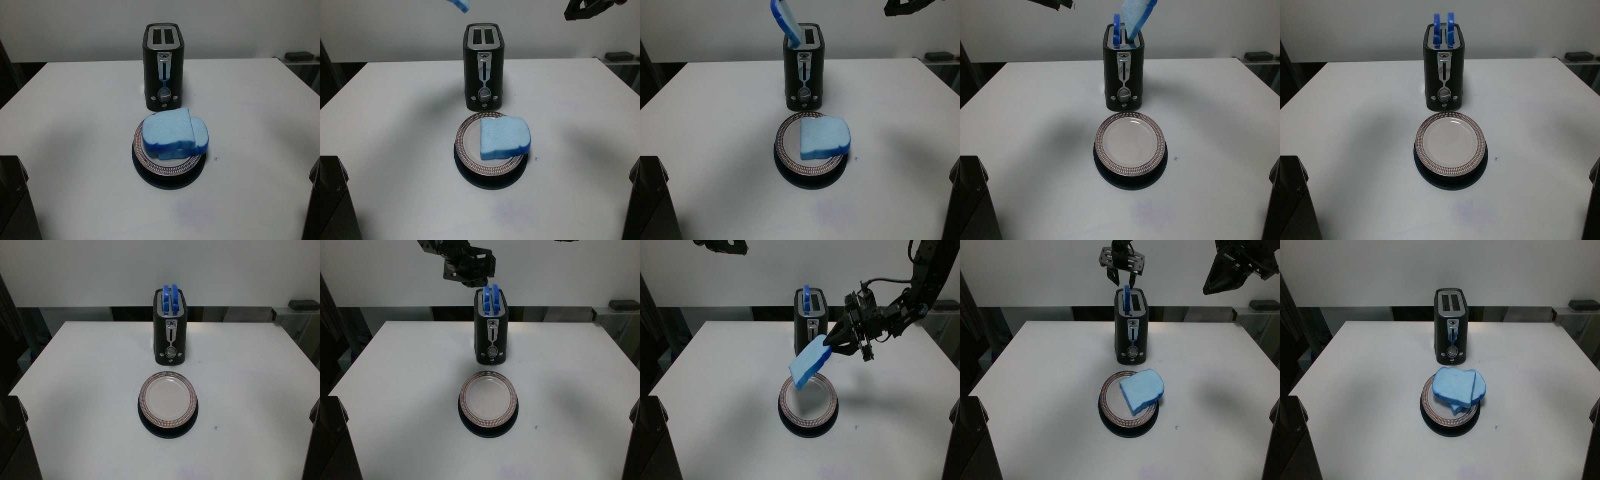
\includegraphics[width=\textwidth]{figs/fig_dataset.jpg}
	\caption{Top-camera views of the ALOHA toaster task. Upper row: insertion, where the robot takes the two foam bread slices from a plate one after the other and lets each fall into a toaster slot. Lower row: removal, where it pulls the slices out and returns them to the plate. The two tasks traverse the same scene states in reverse order.}
	\label{f:dataset}
\end{figure*}

\subsection{Data}
The dataset consists of 100 real bimanual recordings collected with ALOHA~\cite{zhao2023aloha}, a platform with two 6-DoF arms and parallel grippers that logs 14-D joint-space actions at 50\,Hz and three RGB streams (one overhead, one per wrist) at $480\times848$ (Fig.~\ref{f:dataset}).
Every recording is 25\,s long, i.e.\ 1,250 control steps.
The 50 \textbf{insertion} and 50 \textbf{removal} recordings visit three shared scene states in opposite orders: both slices on the plate, one slice in the toaster, and both slices in the toaster.
One additional insertion recording with no joint motion was excluded.
Both regimes that {\method} distinguishes occur in this task: moving a grasped slice is quasi-static and almost reversible, whereas the gravity-driven drop into a slot cannot be undone by reversing the motion.

We compute features at 10\,Hz and let one model step cover 0.5\,s, i.e.\ 50 steps per recording.
All five phase offsets of a recording are used for training, and offset 0 for evaluation.
For each direction we run 5-fold cross-validation with folds formed from whole recordings.
Training never sees joint actions; the sole exception is proprioceptive joint speed, from which the slowest 15\% of steps define the anchor set $\mathcal{N}$.
Gripper positions serve only to locate releases during evaluation; a release is counted when a gripper opens beyond 0.9 after holding an object ($0.05<g<0.9$) for at least 1\,s, a rule that yields exactly two releases in 41 of 50 insertion and 49 of 50 removal recordings.
Detection uses every held-out recording with all the releases the rule finds, which gives 93 post-release steps against 810 carrying steps for insertion and 103 against 898 for removal, pooled over the five folds.
The drop is triggered by the agent opening the gripper and completes within a fraction of one 0.5\,s step; apart from such events the scene is static unless the robot moves it.

\subsection{Representation and Training}
Frames from the top camera are resized to $224\times392$ and encoded by a frozen DINOv2 ViT-S/14~\cite{oquab2024dinov2}.
We concatenate the CLS token (384-D) with a $2\times4$ average-pooled patch grid (3,072-D), standardise, and reduce to 128 dimensions by PCA fitted on training episodes.
Throughout, $o_t$ denotes these 128-D features: the decoder reconstructs features rather than pixels, and all errors are measured in this feature space.
A feature check confirms that this representation encodes the scene state: a linear probe decodes the three scene stages with 97.5\% balanced accuracy (chance 33.3\%; \ref{a:dev}).
The head $\phi$ and decoder are two-layer MLPs with 256 hidden units, $d=64$ and $m=16$.
$K(z)$ is computed with a batched matrix exponential based on scaling and squaring~\cite{higham2005scaling}.
Encoder, decoder and training budget are identical across models: 4,000 Adam updates with batches of 512, learning rate $10^{-3}$, $\lambda_b=\lambda_r=\lambda_a=1$ and $\lambda_v=10^{-3}$.
Each fold takes about ten minutes on one A100 GPU.
Table~\ref{t:main} uses one training seed per fold. \todo{replace with means over three seeds per fold (code/run\_all.sh).}

\subsection{Baselines and Ablations}
\textbf{LAM}~\cite{schmidt2024lapo} uses an MLP forward model and a separate MLP backward model trained on time-reversed clips; its reverse action is the IDM applied to the swapped pair.
\textbf{Sign-reversal LAM}~\cite{tang2026alam} uses one shared MLP forward model, $\zb=-z$, and decodes swapped pairs with the forward model.
\textbf{{\method} w/o anchor} drops the anchor term.
Three Koopman ablations isolate the operator form, the reversal loss and the drift: \textbf{{\method}-SR} decodes the swapped pair under $+G_0$ instead of $-G_0$ and is the model of Proposition~\ref{p:signrev}; \textbf{{\method} w/o reversal} sets $\lambda_r=0$; and \textbf{{\method}, $G_0=0$} removes the drift generator.
The \textbf{two-direction reference} is {\method} trained on both directions.
It sees the test task during training and, in the rollout and alignment metrics, uses the IDM's actions on the test recording itself rather than derived reverse actions, so it is a reference, not an upper bound.

\subsection{Evaluation Protocol}
Models fitted to insertion are evaluated on removal, written I$\to$R; the opposite assignment is written R$\to$I.
Errors are relative to predicting no change, $\|\hat o-o\|^2/\|o_{\mathrm{prev}}-o\|^2$, so 1.0 means no better than copying the current frame.
\begin{enumerate}
	\item \textbf{Forward and backward error}, measured on held-out recordings of the direction used for training. Because the IDM sees $o_{t+1}$, these errors measure reconstruction through the latent-action bottleneck rather than open-loop prediction.
	\item \textbf{End-distance ratio}: starting from a test recording of the opposite task, we roll out the reverse actions derived from a held-out training recording and divide the final distance to the target-stage prototype by the initial one, with distances between decoded features; a ratio below 1 indicates that the rollout moved toward the target. We also report \textbf{stage reach}, the fraction of rollouts that end nearer the target stage than the start stage. A dissipative drift contracts any rollout, so a ratio below 1 can arise without any reversal; as null references we roll out from the same start with zero actions, with random actions drawn from a Gaussian fitted to the training actions, and with the forward actions in their original order.
	\item \textbf{Action alignment}: the cosine between the derived reverse actions and the latent actions the IDM assigns to real reverse recordings, after alignment with dynamic time warping. Because time warping maximises similarity, we also align the derived actions with a time-permuted copy of the real reverse actions.
	\item \textbf{Joint-probe error}: a linear probe from $z$ to 14-D joint deltas, fitted on the training direction and scored on time-warped real reverse actions; as a reference we score negated, time-reversed joint deltas.
	\item \textbf{Reversibility AUROC} of $\kappa_t$ for separating the 0.5\,s after each release from grasped carrying, on held-out recordings of the training direction: for I$\to$R these are insertions, where releases drop slices into the slots, and for R$\to$I removals, where releases put slices on the plate. For LAM baselines we use the condition number of the forward-model Jacobian, which, unlike $\kappa_t$, depends on the state. We also score $\klin_t$, $\rho_t$, $\varepsilon_t$ and four simple detectors ($\|z_t\|$, the feature change $\|o_{t+1}-o_t\|$, arm joint speed and a gripper-opening indicator), against all carrying steps and against matched carrying steps, the three nearest to each post-release step in arm joint speed (the agent's motion) or in feature change (the total motion).
	\item \textbf{Few-shot error}: forward error on the opposite task once the IDM alone, or for Koopman models the IDM and $G_0$, has been fine-tuned on $k\in\{0,1,3,5\}$ recordings.
	\item \textbf{Drift residual} $\varepsilon$ of Eq.~(\ref{e:residual}), with the analytic reference of Remark~\ref{r:eps} and a random drift generator of the same structure and norm, and the per-transition residual $\varepsilon_t$.
	\item \textbf{Undo success}: the fraction of post-release and carrying transitions for which the state-specific undo of Eq.~(\ref{e:undoss}) returns to within half a step, $\|D(K(\zss_t)s_{t+1})-o_t\|<0.5\,\|o_{t+1}-o_t\|$, in one step and with a three-step plan.
	\item \textbf{Drift absorption}: the AUROC of a logistic probe from $z_t$ to the post-release label, fitted on training recordings.
\end{enumerate}
All models of one direction share the test folds, so we compare them fold by fold with paired $t$-tests and report how many folds favour each model; with five folds a two-sided Wilcoxon signed-rank test cannot reach $p<0.05$.

% =====================================================================
\section{Results} \label{s:results}

\begin{figure*}[t]
	\centering
	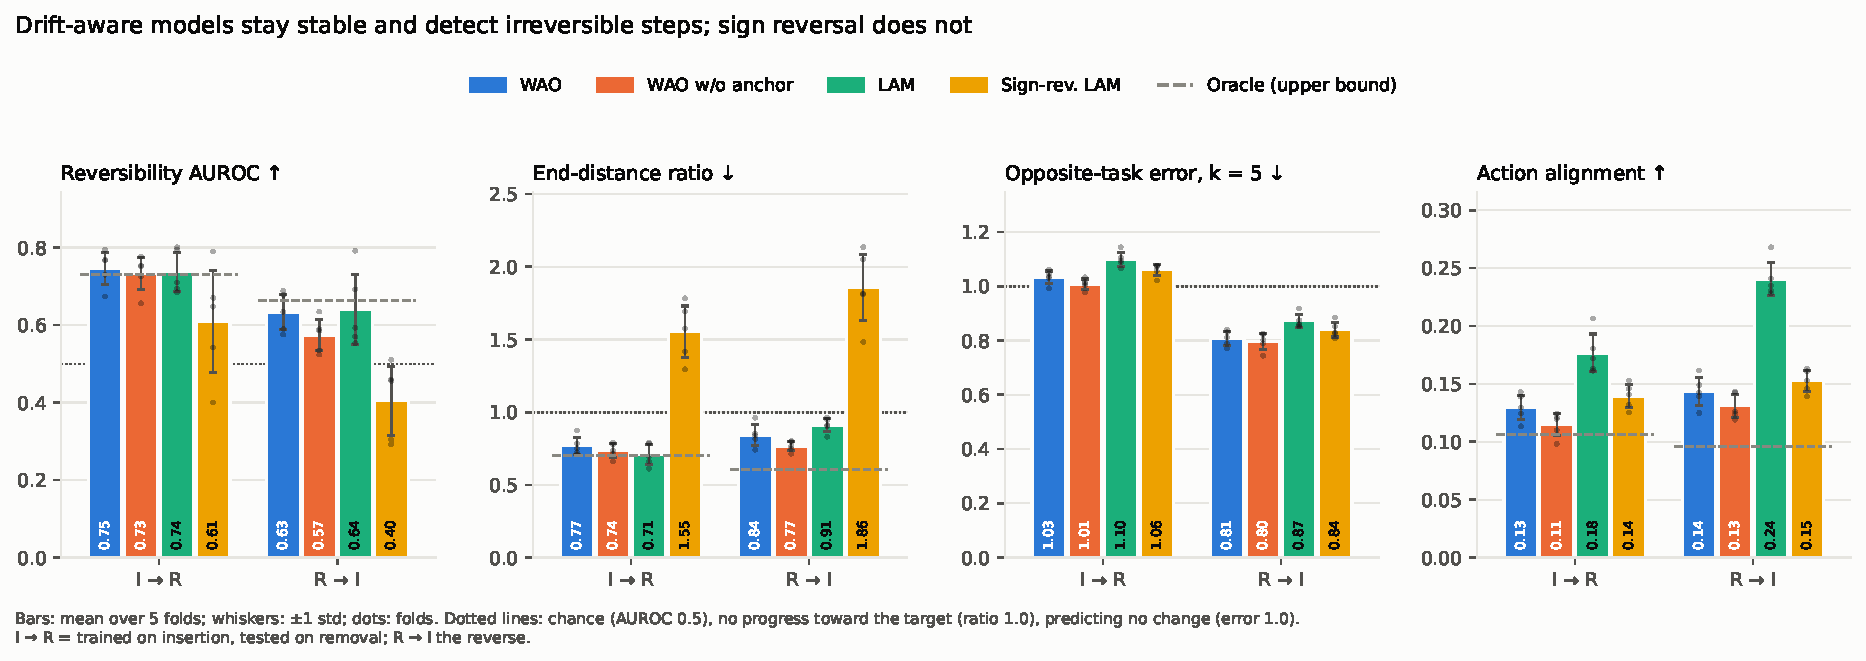
\includegraphics[width=\textwidth]{figs/fig_compare_bars.pdf}
	\caption{Main metrics as mean $\pm$ one standard deviation across the 5 folds, with individual folds shown as dots. Dotted reference lines indicate chance level (AUROC 0.5), no movement toward the target (ratio 1.0) and the no-change predictor (error 1.0); the dashed line marks the two-direction reference, which is also trained on the test direction and is not an upper bound.}
	\label{f:bars}
\end{figure*}

\begin{table*}
	\centering
	\caption{Cross-validated results (mean $\pm$ standard deviation over 5 folds). I$\to$R denotes training on insertion and testing on removal, R$\to$I the opposite. Errors are normalised by the no-change predictor. For forward error, backward error, reversibility AUROC and drift residual, the direction names the training task, evaluated on its held-out recordings. Bold marks the best non-reference entry in each row; the two-direction reference is trained on both directions and is worse than other models on action alignment, joint-probe error and I$\to$R AUROC, so it is not an upper bound. \todo{replace with means over folds and seeds.}}
	\label{t:main}
	\footnotesize
	\setlength{\tabcolsep}{3.2pt}
	\begin{tabular}{llccccc}
		\toprule
		Metric & Dir. & LAM & Sign-rev. LAM & {\method} w/o anchor & {\method} & Two-dir. ref. \\
		\midrule
		\multirow{2}{*}{Forward error $\downarrow$} & I$\to$R & 0.222$\pm$0.011 & \textbf{0.219}$\pm$0.010 & 0.222$\pm$0.011 & 0.230$\pm$0.010 & 0.225$\pm$0.009 \\
		 & R$\to$I & 0.228$\pm$0.007 & \textbf{0.225}$\pm$0.007 & 0.227$\pm$0.006 & 0.234$\pm$0.006 & 0.237$\pm$0.006 \\
		\multirow{2}{*}{Backward error $\downarrow$} & I$\to$R & 0.226$\pm$0.011 & \textbf{0.221}$\pm$0.010 & 0.224$\pm$0.010 & 0.233$\pm$0.010 & 0.226$\pm$0.009 \\
		 & R$\to$I & 0.230$\pm$0.008 & \textbf{0.226}$\pm$0.007 & 0.228$\pm$0.006 & 0.235$\pm$0.006 & 0.236$\pm$0.006 \\
		\multirow{2}{*}{End-distance ratio $\downarrow$} & I$\to$R & \textbf{0.709}$\pm$0.069 & 1.552$\pm$0.178 & 0.736$\pm$0.047 & 0.769$\pm$0.058 & 0.702$\pm$0.044 \\
		 & R$\to$I & 0.911$\pm$0.046 & 1.860$\pm$0.228 & \textbf{0.766}$\pm$0.032 & 0.842$\pm$0.071 & 0.604$\pm$0.015 \\
		\multirow{2}{*}{Stage reach $\uparrow$} & I$\to$R & \textbf{0.96}$\pm$0.08 & 0.94$\pm$0.08 & 0.90$\pm$0.20 & 0.84$\pm$0.19 & 0.98$\pm$0.04 \\
		 & R$\to$I & 0.28$\pm$0.23 & 0.60$\pm$0.31 & \textbf{0.72}$\pm$0.17 & 0.58$\pm$0.25 & 1.00$\pm$0.00 \\
		\multirow{2}{*}{Action alignment $\uparrow$} & I$\to$R & \textbf{0.177}$\pm$0.016 & 0.139$\pm$0.010 & 0.115$\pm$0.010 & 0.130$\pm$0.011 & 0.106$\pm$0.048 \\
		 & R$\to$I & \textbf{0.241}$\pm$0.014 & 0.153$\pm$0.009 & 0.131$\pm$0.010 & 0.144$\pm$0.012 & 0.096$\pm$0.052 \\
		\multirow{2}{*}{Joint-probe error $\downarrow$} & I$\to$R & 1.191$\pm$0.035 & \textbf{1.078}$\pm$0.024 & 1.088$\pm$0.022 & 1.094$\pm$0.023 & 1.225$\pm$0.046 \\
		 & R$\to$I & 1.196$\pm$0.048 & \textbf{1.076}$\pm$0.049 & 1.096$\pm$0.055 & 1.107$\pm$0.053 & 1.270$\pm$0.037 \\
		\multirow{2}{*}{Reversibility AUROC $\uparrow$} & I$\to$R & 0.737$\pm$0.050 & 0.610$\pm$0.131 & 0.733$\pm$0.042 & \textbf{0.747}$\pm$0.042 & 0.731$\pm$0.033 \\
		 & R$\to$I & \textbf{0.640}$\pm$0.090 & 0.404$\pm$0.089 & 0.574$\pm$0.040 & 0.633$\pm$0.045 & 0.664$\pm$0.041 \\
		\multirow{2}{*}{Few-shot error, $k=5$ $\downarrow$} & I$\to$R & 1.099$\pm$0.026 & 1.060$\pm$0.021 & \textbf{1.008}$\pm$0.019 & 1.033$\pm$0.023 & -- \\
		 & R$\to$I & 0.872$\pm$0.024 & 0.840$\pm$0.027 & \textbf{0.796}$\pm$0.030 & 0.808$\pm$0.026 & -- \\
		\multirow{2}{*}{Drift residual $\varepsilon$} & I$\to$R & -- & -- & 0.997$\pm$0.001 & 0.988$\pm$0.005 & 0.991$\pm$0.003 \\
		 & R$\to$I & -- & -- & 0.997$\pm$0.001 & 0.991$\pm$0.001 & 0.991$\pm$0.002 \\
		\bottomrule
	\end{tabular}
\end{table*}


\begin{table*}
	\centering
	\caption{Fold-level paired comparison of {\method} with each baseline (from the runs of Table~\ref{t:main}). $\Delta$: mean $\pm$ standard deviation over the 5 folds of {\method} minus the baseline; wins: folds in which {\method} is better; $p$: paired $t$-test. With five folds a two-sided Wilcoxon test cannot reach $p<0.05$ (its minimum is 0.0625).}
	\label{t:paired}
	\footnotesize
	\setlength{\tabcolsep}{3.5pt}
	\begin{tabular}{llcccccc}
		\toprule
		& & \multicolumn{3}{c}{I$\to$R} & \multicolumn{3}{c}{R$\to$I} \\
		\cmidrule(r){3-5} \cmidrule(l){6-8}
		Baseline & Metric & $\Delta$ & wins & $p$ & $\Delta$ & wins & $p$ \\
		\midrule
		\multirow{4}{*}{LAM} & End-distance ratio $\downarrow$ & +0.060$\pm$0.076 & 1/5 & 0.150 & -0.069$\pm$0.127 & 4/5 & 0.289 \\
		 & Reversibility AUROC $\uparrow$ & +0.009$\pm$0.036 & 2/5 & 0.599 & -0.007$\pm$0.093 & 3/5 & 0.878 \\
		 & Few-shot error, $k=5$ $\downarrow$ & -0.066$\pm$0.016 & 5/5 & $<$0.001 & -0.064$\pm$0.030 & 5/5 & 0.008 \\
		 & Action alignment $\uparrow$ & -0.047$\pm$0.010 & 0/5 & $<$0.001 & -0.097$\pm$0.017 & 0/5 & $<$0.001 \\
		\midrule
		\multirow{4}{*}{Sign-rev. LAM} & End-distance ratio $\downarrow$ & -0.784$\pm$0.158 & 5/5 & $<$0.001 & -1.018$\pm$0.295 & 5/5 & 0.002 \\
		 & Reversibility AUROC $\uparrow$ & +0.137$\pm$0.119 & 5/5 & 0.062 & +0.229$\pm$0.096 & 5/5 & 0.006 \\
		 & Few-shot error, $k=5$ $\downarrow$ & -0.027$\pm$0.012 & 5/5 & 0.007 & -0.031$\pm$0.018 & 5/5 & 0.018 \\
		 & Action alignment $\uparrow$ & -0.010$\pm$0.002 & 0/5 & $<$0.001 & -0.009$\pm$0.010 & 1/5 & 0.110 \\
		\midrule
		\multirow{4}{*}{{\method} w/o anchor} & End-distance ratio $\downarrow$ & +0.033$\pm$0.079 & 2/5 & 0.408 & +0.076$\pm$0.097 & 1/5 & 0.154 \\
		 & Reversibility AUROC $\uparrow$ & +0.014$\pm$0.005 & 5/5 & 0.004 & +0.060$\pm$0.018 & 5/5 & 0.002 \\
		 & Few-shot error, $k=5$ $\downarrow$ & +0.025$\pm$0.011 & 0/5 & 0.006 & +0.012$\pm$0.010 & 1/5 & 0.066 \\
		 & Action alignment $\uparrow$ & +0.015$\pm$0.003 & 5/5 & $<$0.001 & +0.013$\pm$0.006 & 5/5 & 0.011 \\
		\bottomrule
	\end{tabular}
\end{table*}

Fig.~\ref{f:bars} and Table~\ref{t:main} report the cross-validation outcome, and Table~\ref{t:paired} compares {\method} with the baselines fold by fold.
One-step prediction is of similar quality for every model (forward error 0.219--0.237), and the backward error of {\method}, computed with the exact inverse of Proposition~\ref{p:inverse}, is essentially the same as its forward error, as the theory implies.
The exact inverse does not make the backward step more accurate, however: the plain LAM's separately trained backward model reaches 0.226 and 0.230 against 0.233 and 0.235 for {\method}, and {\method}'s forward error is the highest of the four models in every fold, by 0.006--0.011; the value of the exact inverse is that it costs no parameters.
The differences therefore lie in the reverse direction.

\subsection{Sign Reversal in an MLP Model Diverges}
Only the sign-reversal LAM produces diverging reverse rollouts: they finish 1.55 and 1.86 times farther from the target than where they began, above 1.29 in every fold, and its reversibility AUROC drops to 0.61 and 0.40.
Every Koopman model keeps the end-distance ratio under 1.0 and attains an AUROC between 0.57 and 0.75.
The plain LAM, which has no reversal constraint at all, is equally stable (0.71 and 0.91; the paired difference to {\method} is not significant in either direction, Table~\ref{t:paired}) and detects drops equally well.
The result therefore shows that sign reversal in an MLP model fails on this task; it does not by itself show that the drift-aware loss is what prevents the failure.
Proposition~\ref{p:signrev} predicts the failure for sign reversal in Koopman form, which the MLP baseline is not, and its divergence may also come from evaluating the MLP forward model at $-z$, outside the actions seen in training.
The Koopman ablations of Table~\ref{t:ablation} separate these explanations. \todo{report end distance and AUROC of {\method}-SR, {\method} w/o reversal and {\method} with $G_0=0$.}
A ratio below 1 is also evidence of reversal only if it is clearly below that of the null rollouts in Table~\ref{t:undo}. \todo{report.}
In the controlled study of Section~\ref{s:toy}, where the drift is known, the Koopman sign-reversal model absorbs more of the passive motion than {\method} (0.81 against 0.70) and its reverse action $-z$ undoes reversible steps worse (1.22 against 0.76 step lengths), as Proposition~\ref{p:signrev} predicts.

\begin{table*}
	\centering
	\caption{Koopman ablations on the robot data, mean $\pm$ standard deviation over folds. Rows for {\method}, {\method} w/o anchor, LAM and sign-rev.\ LAM repeat Table~\ref{t:main}. Absorption: AUROC of a logistic probe from $z_t$ to the post-release label (lower means that less of the drop is written into the action). $^\dagger$Condition number of the forward-model Jacobian, which depends on the state. \textcolor{red}{tbd}: requires the runs of code/run\_all.sh.}
	\label{t:ablation}
	\footnotesize
	\setlength{\tabcolsep}{3.2pt}
	\begin{tabular}{lcccccccc}
		\toprule
		& \multicolumn{2}{c}{End-distance ratio $\downarrow$} & \multicolumn{2}{c}{Reversibility AUROC $\uparrow$} & \multicolumn{2}{c}{Few-shot error, $k=5$ $\downarrow$} & \multicolumn{2}{c}{Absorption probe} \\
		\cmidrule(lr){2-3} \cmidrule(lr){4-5} \cmidrule(lr){6-7} \cmidrule(lr){8-9}
		Model & I$\to$R & R$\to$I & I$\to$R & R$\to$I & I$\to$R & R$\to$I & I$\to$R & R$\to$I \\
		\midrule
		{\method} & 0.769$\pm$0.058 & 0.842$\pm$0.071 & 0.747$\pm$0.042 & 0.633$\pm$0.045 & 1.033$\pm$0.023 & 0.808$\pm$0.026 & \tbd & \tbd \\
		{\method} w/o anchor & 0.736$\pm$0.047 & 0.766$\pm$0.032 & 0.733$\pm$0.042 & 0.574$\pm$0.040 & 1.008$\pm$0.019 & 0.796$\pm$0.030 & \tbd & \tbd \\
		{\method}-SR ($+G_0$) & \tbd & \tbd & \tbd & \tbd & \tbd & \tbd & \tbd & \tbd \\
		{\method} w/o reversal & \tbd & \tbd & \tbd & \tbd & \tbd & \tbd & \tbd & \tbd \\
		{\method}, $G_0=0$ & \tbd & \tbd & \tbd & \tbd & \tbd & \tbd & \tbd & \tbd \\
		{\method}, $G_0$ fine-tuned & -- & -- & -- & -- & \tbd & \tbd & -- & -- \\
		LAM & 0.709$\pm$0.069 & 0.911$\pm$0.046 & 0.737$\pm$0.050$^\dagger$ & 0.640$\pm$0.090$^\dagger$ & 1.099$\pm$0.026 & 0.872$\pm$0.024 & \tbd & \tbd \\
		Sign-rev. LAM & 1.552$\pm$0.178 & 1.860$\pm$0.228 & 0.610$\pm$0.131$^\dagger$ & 0.404$\pm$0.089$^\dagger$ & 1.060$\pm$0.021 & 0.840$\pm$0.027 & \tbd & \tbd \\
		\bottomrule
	\end{tabular}
\end{table*}

\begin{figure}[t]
	\centering
	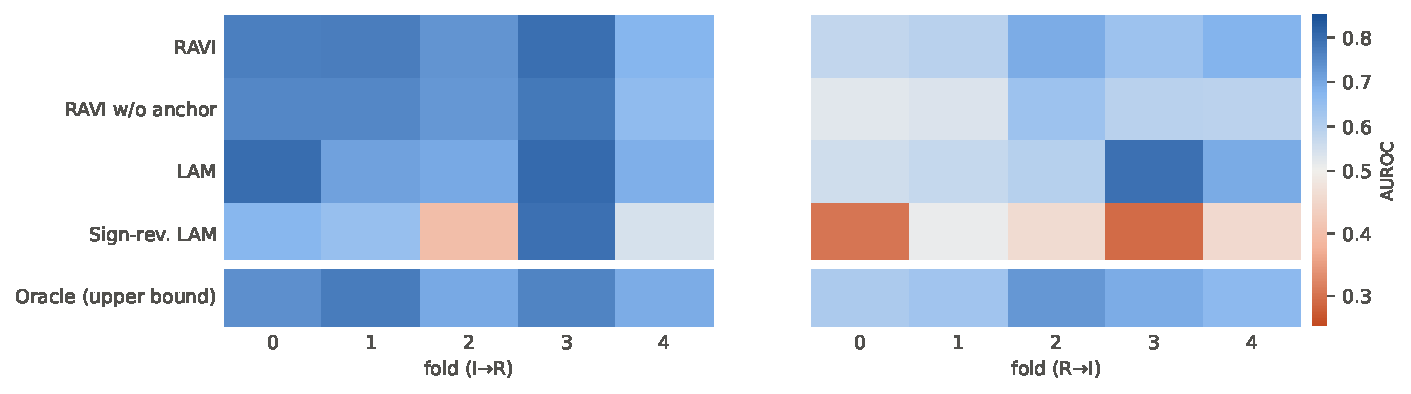
\includegraphics[width=\columnwidth]{figs/fig_auroc_folds_heatmap.pdf}
	\caption{Per-fold reversibility AUROC, with the colour scale centred at chance (0.5). In 4 of the 5 R$\to$I folds the sign-reversal LAM is below chance, while all Koopman models remain above chance in all folds.}
	\label{f:folds}
\end{figure}

\subsection{Detecting Irreversible Moments}
$\kappa_t$ distinguishes the half second following a release, during which a slice drops into a slot or onto the plate, from periods of grasped transport, reaching an AUROC of $0.747\pm0.042$ for I$\to$R and $0.633\pm0.045$ for R$\to$I.
The plain LAM scores 0.737 and 0.640, within one standard deviation of these values, yet only {\method} also supplies reverse actions in closed form.
Fold by fold (Fig.~\ref{f:folds}), sign reversal drops below chance in four of the five R$\to$I folds, whereas no Koopman model ever does.
The anchor helps here: {\method} exceeds {\method} without the anchor in every fold of both directions, by 0.014 and 0.060 (paired $p=0.004$ and $0.002$).
By Corollary~\ref{c:kappa}, however, $\kappa_t$ responds only to the inferred action, so this AUROC may reflect the release motion or the arm's speed rather than the passive drop.
Table~\ref{t:detect} therefore compares $\kappa_t$ with its translation-free and state-dependent variants and with simple detectors, against ordinary and motion-matched negatives. \todo{report whether any score stays above chance against motion-matched negatives and whether it beats the best simple detector.}
The controlled study shows why the control matters: there, $\kappa_t$ separates irreversible from reversible steps with AUROC 0.73 for {\method}, but only 0.50 against reversible steps of the same displacement (Section~\ref{s:toy}); arm speed measures only the agent's motion, so Table~\ref{t:detect} also matches on the feature change.

\begin{table}
	\centering
	\caption{Reversibility AUROC of each score for post-release steps against all carrying steps, and against the three carrying steps nearest to each post-release step in arm joint speed or in feature change $\|o_{t+1}-o_t\|$. $^\dagger$State-dependent Jacobian condition number.}
	\label{t:detect}
	\footnotesize
	\setlength{\tabcolsep}{2.2pt}
	\resizebox{\columnwidth}{!}{%
	\begin{tabular}{lcccccc}
		\toprule
		& \multicolumn{2}{c}{All carrying} & \multicolumn{2}{c}{Same arm speed} & \multicolumn{2}{c}{Same feat.\ change} \\
		\cmidrule(r){2-3} \cmidrule(lr){4-5} \cmidrule(l){6-7}
		Score & I$\to$R & R$\to$I & I$\to$R & R$\to$I & I$\to$R & R$\to$I \\
		\midrule
		$\kappa_t$ ({\method}) & 0.747 & 0.633 & \tbd & \tbd & \tbd & \tbd \\
		$\klin_t$ ({\method}) & \tbd & \tbd & \tbd & \tbd & \tbd & \tbd \\
		$\rho_t$ ({\method}) & \tbd & \tbd & \tbd & \tbd & \tbd & \tbd \\
		$\varepsilon_t$ ({\method}) & \tbd & \tbd & \tbd & \tbd & \tbd & \tbd \\
		Jacobian cond.\ (LAM)$^\dagger$ & 0.737 & 0.640 & \tbd & \tbd & \tbd & \tbd \\
		\midrule
		$\|z_t\|$ ({\method}) & \tbd & \tbd & \tbd & \tbd & \tbd & \tbd \\
		$\|o_{t+1}-o_t\|$ & \tbd & \tbd & \tbd & \tbd & -- & -- \\
		Arm joint speed & \tbd & \tbd & -- & -- & \tbd & \tbd \\
		Gripper opening & \tbd & \tbd & \tbd & \tbd & \tbd & \tbd \\
		\bottomrule
	\end{tabular}}
\end{table}

\subsection{Undo and Drift Residual}
The drift residual is 0.988--0.997 for every Koopman model, the two-direction reference included, so the undo action of Eq.~(\ref{e:undo}) reduces to $-z$ in practice and no state-independent single-step undo exists for the learned operator.
Remark~\ref{r:eps} shows that this value is close to what unrelated actions and drift would give: the analytic reference is at least 0.87 for $m=16$ and $d=64$, and in a development run, weakening the penalty on the symmetric action blocks to $\lambda_v=10^{-5}$ or 0 left the residual at 0.992.
The residual therefore shows that the learned actions cannot cancel the learned drift, not that a drop is irreversible.
Table~\ref{t:undo} adds the random-drift reference, the per-transition residual at drops and during carrying, and the success of state-specific and three-step undo. \todo{report Table~\ref{t:undo}.}
In the controlled study, where part of the drift can be cancelled, the residual is 0.85 for {\method} and 0.52--0.61 without the reversal loss or the anchor, below a random-drift reference of 0.97, and the drift correction improves the undo action (Section~\ref{s:toy}).

\begin{table}
	\centering
	\caption{Null references and undo diagnostics for {\method}. Values without \textcolor{red}{tbd} repeat Table~\ref{t:main}. Undo success: fraction of transitions returned to within half a step in decoded features (post-release / carrying).}
	\label{t:undo}
	\footnotesize
	\setlength{\tabcolsep}{3pt}
	\begin{tabular}{lcc}
		\toprule
		Quantity & I$\to$R & R$\to$I \\
		\midrule
		End-distance ratio, {\method} & 0.769 & 0.842 \\
		\quad null: zero actions & \tbd & \tbd \\
		\quad null: random actions & \tbd & \tbd \\
		\quad null: unreversed forward actions & \tbd & \tbd \\
		Action alignment, {\method} & 0.130 & 0.144 \\
		\quad reference: time-permuted actions & \tbd & \tbd \\
		\midrule
		Drift residual $\varepsilon$, {\method} & 0.988 & 0.991 \\
		\quad analytic reference (Remark~\ref{r:eps}) & $\ge0.87$ & $\ge0.87$ \\
		\quad random $G_0$, matched norm & \tbd & \tbd \\
		$\varepsilon_t$: post-release / carrying & \tbd & \tbd \\
		Undo success, one step & \tbd & \tbd \\
		Undo success, three steps & \tbd & \tbd \\
		$\|A(z_t)\|_2$: median (max) & \tbd & \tbd \\
		\bottomrule
	\end{tabular}
\end{table}

\subsection{Transfer to the Opposite Task}

\begin{figure}[t]
	\centering
	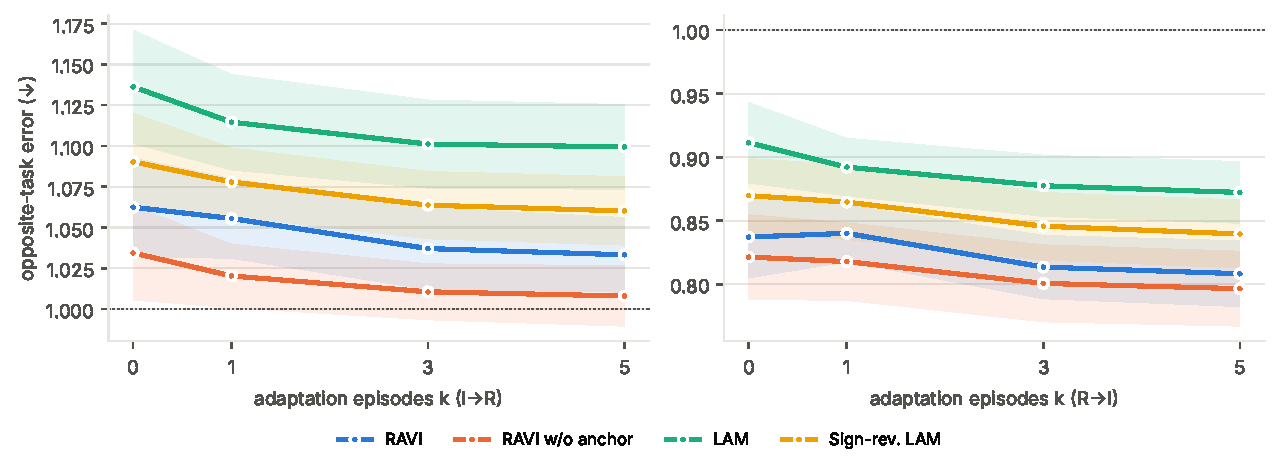
\includegraphics[width=\columnwidth]{figs/fig_fewshot_curves.pdf}
	\caption{Forward error on the opposite task after only the IDM is fine-tuned on $k$ recordings; bands show one standard deviation.}
	\label{f:fewshot}
\end{figure}

When $\phi$ and $G_0$ are frozen and only the IDM is adapted, the two {\method} variants give the smallest opposite-task error for every $k$ and in both directions (Fig.~\ref{f:fewshot}).
For $k=5$, {\method} without the anchor attains 1.008 on I$\to$R and 0.796 on R$\to$I, the anchored variant 1.033 and 0.808, the plain LAM 1.099 and 0.872, and sign reversal 1.060 and 0.840.
{\method} is better than the plain LAM in every fold of both directions (paired $p=0.001$ and $0.008$), and the anchor costs transfer: {\method} without it is better in all five I$\to$R folds ($p=0.006$) and in four of five R$\to$I folds ($p=0.066$).
The gap to the LAM baselines is present already at $k=0$, before any adaptation, so it does not by itself show that the shared drift is what transfers; fine-tuning $G_0$ as well, and removing it, test this (Table~\ref{t:ablation}). \todo{report.}
For I$\to$R the error stays at or above the no-change level of 1.0 even after five recordings, so no model predicts removal from insertion data better than copying the current frame; in that direction the advantage is a smaller deficit, not useful prediction.

\subsection{Controlled Study with Known Drift} \label{s:toy}
To test the theory where the ground truth is known, we simulate a point $p\in\R^2$ with $p_{t+1}=p_t+\Delta t\,(f(p_t)+u_t)$, $\Delta t=0.1$ and actions $u\in[-1,1]^2$, observed only through a fixed random two-layer $\tanh$ lift to 32 dimensions.
The drift $f(p)=g-k\,w(p)\,(p-c)$ combines a constant pull $g=(0,-0.5)$ with a dissipative well of radius 1 around $c=(0,-1)$, where $w$ is a smooth indicator and $k=3$, so the scene settles on its own inside the well.
The dynamics are first order, as Definition~\ref{d:trev} assumes, and every transition has a unique one-step undo action $u^*=(p_t-p_{t+1})/\Delta t-f(p_{t+1})$; we call a transition reversible if the agent can execute it, $\|u^*\|_\infty\le2$, which holds everywhere outside the well and fails for 21.7\% of all transitions.
Idle steps ($u=0$) occur with probability 0.15 and, as on the robot, the anchor sees only those outside the well.
All seven models use the architecture of Section~\ref{s:method} with $d=8$, $m=2$ and 3,000 training steps and are evaluated on 6,000 fresh transitions, over three seeds (Table~\ref{t:toyd}).
Latent actions are mapped to real actions by a linear probe fitted on labeled transitions, which fixes the gauge, and undo actions are executed in the simulator.

\begin{table*}
	\centering
	\caption{Controlled study with known dissipative drift (mean $\pm$ standard deviation over 3 seeds). Absorbed drift: size of the action that the probe reads from $z_t$ on idle steps inside the well, where the true action is zero, relative to the mean action size. AUROC: irreversible against reversible steps, either all of them or the three nearest in displacement $\|p_{t+1}-p_t\|$. Return: simulator distance to $p_t$ after executing the undo action, divided by the step length (median). Model-independent references: AUROC of the feature change 0.93 (all) and 0.60 (equal displacement), of the true drift magnitude 0.99 and 0.99; drift residual of a random generator 0.97; return of the negated true action 1.40 (reversible) and 1.74 (irreversible); best possible return 0 and 0.61.}
	\label{t:toyd}
	\footnotesize
	\setlength{\tabcolsep}{3pt}
	\begin{tabular}{lccccccc}
		\toprule
		& {\method} & w/o anchor & {\method}-SR & w/o reversal & $G_0=0$ & LAM & Sign-rev. LAM \\
		\midrule
		Forward error $\downarrow$ & 0.29$\pm$0.02 & 0.02$\pm$0.01 & 0.30$\pm$0.04 & 0.14$\pm$0.02 & 0.37$\pm$0.07 & 0.02$\pm$0.00 & 0.02$\pm$0.00 \\
		Backward error $\downarrow$ & 0.26$\pm$0.01 & 0.02$\pm$0.01 & 0.19$\pm$0.00 & 0.14$\pm$0.01 & 0.26$\pm$0.02 & 0.02$\pm$0.00 & 0.02$\pm$0.00 \\
		IDM antisymmetry $\cos(\zb,-z)$ & 0.93$\pm$0.04 & 1.00$\pm$0.00 & 0.95$\pm$0.02 & 0.39$\pm$0.04 & 0.96$\pm$0.01 & 0.28$\pm$0.01 & 1.00$\pm$0.00 \\
		Absorbed drift, idle in well $\downarrow$ & 0.70$\pm$0.03 & 0.95$\pm$0.03 & 0.81$\pm$0.03 & 0.79$\pm$0.04 & 0.83$\pm$0.02 & 0.89$\pm$0.02 & 0.94$\pm$0.03 \\
		AUROC of $\kappa_t$, all steps & 0.73$\pm$0.05 & 0.92$\pm$0.01 & 0.84$\pm$0.02 & 0.69$\pm$0.04 & 0.86$\pm$0.02 & 0.78$\pm$0.02 & 0.68$\pm$0.12 \\
		AUROC of $\kappa_t$, equal displacement & 0.50$\pm$0.05 & 0.60$\pm$0.03 & 0.52$\pm$0.05 & 0.38$\pm$0.03 & 0.52$\pm$0.05 & 0.52$\pm$0.01 & 0.56$\pm$0.09 \\
		Drift residual $\varepsilon$ & 0.85$\pm$0.01 & 0.61$\pm$0.04 & 0.86$\pm$0.02 & 0.52$\pm$0.01 & -- & -- & -- \\
		Return, reversible, closed form $\downarrow$ & 0.76$\pm$0.02 & 0.79$\pm$0.02 & 1.22$\pm$0.01 & 0.56$\pm$0.08 & 1.19$\pm$0.01 & 0.53$\pm$0.03 & 0.81$\pm$0.02 \\
		Return, reversible, planned $\downarrow$ & 0.88$\pm$0.02 & 0.76$\pm$0.01 & 0.66$\pm$0.07 & 0.56$\pm$0.02 & 0.82$\pm$0.07 & 0.45$\pm$0.03 & 0.78$\pm$0.02 \\
		Return, irreversible, planned $\downarrow$ & 1.10$\pm$0.02 & 1.36$\pm$0.02 & 1.30$\pm$0.02 & 1.06$\pm$0.04 & 1.33$\pm$0.02 & 1.11$\pm$0.04 & 1.36$\pm$0.02 \\
		\bottomrule
	\end{tabular}
\end{table*}

Three results bear on the claims of this paper.
First, decoding under $-G_0$ reduces drift absorption but does not remove it.
On idle steps inside the well, the probe reads an action of 0.70 of the typical size from the latent action of {\method}, against 0.81 for {\method}-SR, 0.79 without the reversal loss, 0.83 with $G_0=0$ and 0.89--0.95 for the MLP models and for {\method} without the anchor.
Proposition~\ref{p:signrev} predicts the direction of the first comparison, but most of the passive motion still enters the action; the anchor accounts for the larger part of the reduction and costs the Koopman models most of their fit (forward error 0.29 with it, 0.02 without).
Second, $\kappa_t$ detects irreversible steps through motion rather than through irreversibility.
Against all reversible steps its AUROC is 0.68--0.92, but against reversible steps of the same displacement it falls to 0.38--0.60 for every model, while the true drift magnitude stays at 0.99.
Matching on the agent's action alone, the analogue of arm speed on the robot, leaves the AUROC of {\method} at 0.72, so matched negatives must control the total displacement.
The state-dependent alternatives do not help: $\rho_t$ is below chance (0.18--0.34) and $\varepsilon_t$ is inconsistent across variants (0.41--0.82).
Third, the drift correction of the undo action matters where the drift can be cancelled.
On reversible steps, executing {\method}'s closed-form undo $-z-2c$ returns the point to within 0.76 step lengths, against 1.22 for $-z$ in {\method}-SR, 1.19 with $G_0=0$ and 1.40 for negating the true action; the plain LAM's reverse action does better still (0.53), and no model comes close to a perfect return, which the probe ($R^2=0.32$--$0.59$) limits.
On irreversible steps every model stays above 1.0 step lengths, against a best possible 0.61.
Finally, removing the reversal loss lowers the antisymmetry of the IDM from 0.93 to 0.39 cosine, as Remark~\ref{r:reduce} implies, and raises absorption from 0.70 to 0.79; the drift residual is 0.52--0.86 for the variants with a drift generator, below the random-drift reference of 0.97, so here the actions cancel part of the drift.

\subsection{Further Results}
None of the models reproduces the actual reverse joint motion: all joint-probe errors are above 1.0, although each one improves on negated, time-reversed joint deltas (1.58 and 1.53)---evidence that removal is not simply insertion run backward.
\ref{a:cv} gives all metrics at a glance, the few-shot errors at every $k$, per-fold tables and a step-by-step walkthrough of every model variable on a held-out episode.
\ref{a:toy} details the controlled study of Section~\ref{s:toy} and reports an earlier variant with constant drift, where the derived undo action returns the state about four times closer than negating the action.
\ref{a:dev} reports the development runs behind the step size, the generator penalty, the drift fit, the release labels and the feature choice, and \ref{a:impl} lists all implementation settings.


% =====================================================================
\section{Discussion and Limitations} \label{s:discussion}

\paragraph{What the evidence supports.}
The cross-validated results support three claims, each holding fold by fold: Koopman models with a drift generator avoid the divergence and below-chance detection of an MLP sign-reversal model; the condition number of the learned step separates post-release windows from grasped carrying well above chance; and the Koopman variants transfer best to the opposite task when only the IDM is adapted.
In the controlled study with known drift, decoding swapped pairs under $-G_0$ absorbs less passive motion than under $+G_0$, and the drift correction improves the undo action on reversible steps, in line with Propositions~\ref{p:undo} and~\ref{p:signrev}.

\paragraph{What it does not.}
{\method} does not outperform a plain LAM in reversibility detection or in the stability of reverse rollouts, and the plain LAM, which has no reversal constraint, aligns actions better and reaches a lower I$\to$R end distance; the full {\method} is best on only one entry of Table~\ref{t:main}, within one standard deviation.
On the robot data it therefore remains open whether the stability comes from decoding under $-G_0$, from the exact-inverse structure or from the drift generator at all; the Koopman ablations of Table~\ref{t:ablation} address this. \todo{revise once Table~\ref{t:ablation} is filled.}
The robot-idle anchor raises detection in every fold but costs transfer, likely because idle steps rarely coincide with strong drift in this task, so the anchor constrains the gauge where it matters least.
The undo action is limited by a drift residual near 0.99, close to the value expected when actions and drift are unrelated (Remark~\ref{r:eps}); a dropped slice is not undone in one step, and $\zundo$ reduces to $-z$ in practice.
{\method} measures how much drift its actions cannot cancel, but on the robot data this does not yet show whether the residual reflects the physics of the task or the parameterisation.
Insertion-to-removal transfer stays at the no-change level.
In the controlled study, $\kappa_t$ separates irreversible steps only through their larger motion and is at chance against steps of equal displacement, the state-dependent alternatives $\rho_t$ and $\varepsilon_t$ do not detect irreversibility either, and a plain LAM undoes reversible steps better than any Koopman variant; the anchor reduces drift absorption there but costs most of the Koopman models' fit.

\paragraph{Scope.}
The evaluation uses one task, one camera view for the dynamics, a frozen encoder and one training seed per fold. \todo{three seeds once run.}
The latent state is computed from a single frame and its dynamics are first order, so Definition~\ref{d:trev} is time reversal of the learned dynamics, not of the mechanics, and momentum is not represented.
In this task the drop completes within a fraction of one 0.5\,s step and is triggered by the agent opening the gripper, and the scene is otherwise static unless the robot moves it; a constant drift generator applied at every state is a coarse model of such event-triggered passive motion.
The anchor uses proprioceptive joint speed, so the anchored model is not trained from video alone.
The theory assumes generators small enough that the matrix exponential is injective, which should hold for 0.5\,s steps and is checked through $\|A(z_t)\|_2$ in Table~\ref{t:undo}; longer horizons need the same check.

\paragraph{Outlook: deformable objects.}
Folding clothes would be an informative next benchmark, since a single task contains both regimes~\cite{lin2020softgym,lin2021vcd}.
Slow folding motions are close to reversible, but draping and settling after release dissipate energy---their Koopman modes satisfy $|\lambda|<1$---and cloth is typically unfolded by flinging or regrasping rather than by reversing the fold~\cite{ha2021flingbot,avigal2022speedfolding}.
Koopman models already control soft robots~\cite{bruder2019soft}.
Settling continues after the gripper lets go, so cloth also offers passive motion without agent action, which the toaster task lacks.
We expect state-dependent scores such as $\rho_t$ and $\varepsilon_t$ to separate fold and settle phases, and state-specific undo to quantify how much of a fold can be undone in one step.

% =====================================================================
\section{Conclusion} \label{s:conclusion}

Recovering reverse actions from video hinges on telling the agent's effect apart from the scene's autonomous motion.
{\method} expresses this separation with a Koopman operator whose drift generator is distinct from its action generators.
Trained only on forward footage, it delivers an exact backward step in the lifted space, the time-reversal action of the first-order latent dynamics, the undo action and a reversibility score; we proved when each is exact, why sign reversal in Koopman form forces zero drift and why the split between agent and drift must be anchored, and we showed that the score depends only on the inferred action and that a drift residual near 1 is expected when actions and drift are unrelated.
On real bimanual robot data, reverse rollouts of {\method} remained stable where an MLP sign-reversal model diverged, irreversible drops were detected clearly above chance, and transfer to the opposite task was the best among the compared models; a plain LAM, however, was equally stable and equally good at detection, and a dropped object still could not be restored in one step.
In a controlled study with known drift, decoding under the reversed drift absorbed less passive motion than sign reversal and the drift correction improved the undo action, but the reversibility score tracked motion rather than irreversibility, which calls for state-dependent scores.
Multi-step undo, state-dependent reversibility scores, velocity-aware latent states and deformable objects are the next steps.

\ack{To be added after review.}

\bibliographystyle{IEEEtran}
\bibliography{ravi}

\clearpage
% =====================================================================
\appendix

\section{Additional Cross-Validation Results} \label{a:cv}

Unless noted, every result in this appendix is taken from the 50 cross-validation runs of Section~\ref{s:results} (5 folds, 5 models, 2 directions).

\subsection{All Metrics at a Glance}

\begin{figure*}[t]
	\centering
	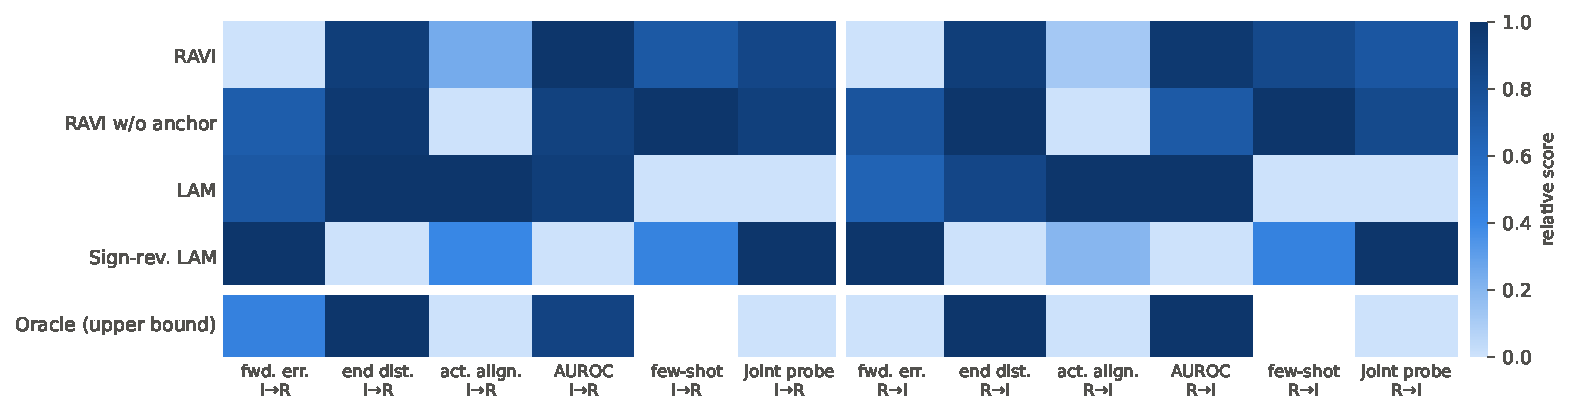
\includegraphics[width=0.92\textwidth]{figs/fig_scorecard_heatmap.pdf}
	\caption{Every metric for every model and both directions. Each cell gives the raw mean over 5 folds; shading is normalised within each column over the four non-reference models, which can make small differences look large.}
	\label{f:scorecard}
\end{figure*}

Fig.~\ref{f:scorecard} shows that no model wins everywhere.
The {\method} variants lead on end distance for R$\to$I and on transfer; the plain LAM leads on action alignment, on end distance for I$\to$R and, narrowly, on R$\to$I detection; and the sign-reversal LAM has the lowest joint-probe error despite its divergent rollouts.
No model reproduces the true reverse joint motion: all probe errors are above 1.0, although every model improves on negated, time-reversed joint deltas, showing that removal is not insertion run backward.

\subsection{Few-Shot Adaptation at Every $k$}

\begin{table*}
	\centering
	\caption{Opposite-task forward error once only the IDM has been fine-tuned on $k$ recordings of the opposite task (mean $\pm$ standard deviation over 5 folds, normalised by the no-change predictor). Bold marks the best entry per column.}
	\label{t:fewshot}
	\footnotesize
	\setlength{\tabcolsep}{4pt}
	\begin{tabular}{lcccccccc}
		\toprule
		& \multicolumn{4}{c}{I$\to$R} & \multicolumn{4}{c}{R$\to$I} \\
		\cmidrule(r){2-5} \cmidrule(l){6-9}
		Model & $k=0$ & $k=1$ & $k=3$ & $k=5$ & $k=0$ & $k=1$ & $k=3$ & $k=5$ \\
		\midrule
		LAM & 1.136$\pm$0.035 & 1.115$\pm$0.029 & 1.101$\pm$0.027 & 1.099$\pm$0.026 & 0.911$\pm$0.032 & 0.892$\pm$0.023 & 0.878$\pm$0.024 & 0.872$\pm$0.024 \\
		Sign-rev. LAM & 1.090$\pm$0.030 & 1.078$\pm$0.021 & 1.064$\pm$0.021 & 1.060$\pm$0.021 & 0.870$\pm$0.029 & 0.865$\pm$0.029 & 0.846$\pm$0.027 & 0.840$\pm$0.027 \\
		{\method} w/o anchor & \textbf{1.034}$\pm$0.029 & \textbf{1.020}$\pm$0.020 & \textbf{1.011}$\pm$0.017 & \textbf{1.008}$\pm$0.019 & \textbf{0.821}$\pm$0.033 & \textbf{0.818}$\pm$0.031 & \textbf{0.801}$\pm$0.030 & \textbf{0.796}$\pm$0.030 \\
		{\method} & 1.062$\pm$0.030 & 1.056$\pm$0.024 & 1.037$\pm$0.025 & 1.033$\pm$0.023 & 0.837$\pm$0.032 & 0.840$\pm$0.022 & 0.813$\pm$0.025 & 0.808$\pm$0.026 \\
		\bottomrule
	\end{tabular}
\end{table*}

Table~\ref{t:fewshot} lists the few-shot errors behind Fig.~\ref{f:fewshot}.
The two {\method} variants are the two best models at every $k$ in both directions, and the gap to the LAM baselines is present already at $k=0$, before any adaptation.

\subsection{Reference Values}
The negated, time-reversed joint deltas of the paired forward recording give joint-probe errors of $1.583\pm0.090$ (I$\to$R) and $1.533\pm0.044$ (R$\to$I), higher than those of every learned model in Table~\ref{t:main}.
Stage reach is noisy with 10 test episodes per fold (Table~\ref{t:main}); the end-distance ratio is the more stable rollout measure.

\subsection{Per-Fold Results}
Tables~\ref{t:perfoldI} and~\ref{t:perfoldR} give the per-fold values of the main reverse-direction metrics.
The sign-reversal LAM has an end-distance ratio above 1.29 in every fold of both directions, while every Koopman model stays below 1.0 in every fold.

\begin{table*}
\centering
\caption{Per-fold results, trained on insertion, tested on removal (I$\to$R). Folds are disjoint sets of test episodes.}
\label{t:perfoldI}
\footnotesize
\setlength{\tabcolsep}{4pt}
\begin{tabular}{llccccc}
\toprule
Quantity & Method & F0 & F1 & F2 & F3 & F4 \\
\midrule
\multirow{5}{*}{End-distance ratio $\downarrow$} & LAM & 0.611 & 0.696 & 0.785 & 0.789 & 0.662 \\
 & Sign-rev. LAM & 1.694 & 1.573 & 1.296 & 1.783 & 1.415 \\
 & \method{} w/o anchor & 0.790 & 0.779 & 0.736 & 0.716 & 0.660 \\
 & \method & 0.783 & 0.725 & 0.752 & 0.873 & 0.710 \\
 & Two-dir. ref. & 0.697 & 0.666 & 0.642 & 0.756 & 0.747 \\
\midrule
\multirow{5}{*}{Reversibility AUROC $\uparrow$} & LAM & 0.795 & 0.710 & 0.695 & 0.801 & 0.685 \\
 & Sign-rev. LAM & 0.670 & 0.647 & 0.400 & 0.790 & 0.542 \\
 & \method{} w/o anchor & 0.752 & 0.753 & 0.725 & 0.777 & 0.656 \\
 & \method & 0.767 & 0.768 & 0.730 & 0.794 & 0.673 \\
 & Two-dir. ref. & 0.740 & 0.772 & 0.696 & 0.758 & 0.691 \\
\midrule
\multirow{5}{*}{Action alignment $\uparrow$} & LAM & 0.181 & 0.161 & 0.207 & 0.172 & 0.163 \\
 & Sign-rev. LAM & 0.146 & 0.125 & 0.153 & 0.141 & 0.132 \\
 & \method{} w/o anchor & 0.121 & 0.098 & 0.124 & 0.120 & 0.110 \\
 & \method & 0.139 & 0.113 & 0.143 & 0.130 & 0.125 \\
 & Two-dir. ref. & 0.106 & 0.194 & 0.077 & 0.102 & 0.052 \\
\midrule
\multirow{4}{*}{Few-shot error, $k=5$ $\downarrow$} & LAM & 1.088 & 1.094 & 1.065 & 1.144 & 1.106 \\
 & Sign-rev. LAM & 1.071 & 1.056 & 1.021 & 1.076 & 1.076 \\
 & \method{} w/o anchor & 1.004 & 1.015 & 0.976 & 1.033 & 1.011 \\
 & \method & 1.046 & 1.035 & 0.993 & 1.062 & 1.030 \\
\bottomrule
\end{tabular}
\end{table*}

\begin{table*}
\centering
\caption{Per-fold results, trained on removal, tested on insertion (R$\to$I). Folds are disjoint sets of test episodes.}
\label{t:perfoldR}
\footnotesize
\setlength{\tabcolsep}{4pt}
\begin{tabular}{llccccc}
\toprule
Quantity & Method & F0 & F1 & F2 & F3 & F4 \\
\midrule
\multirow{5}{*}{End-distance ratio $\downarrow$} & LAM & 0.948 & 0.905 & 0.911 & 0.962 & 0.830 \\
 & Sign-rev. LAM & 1.817 & 2.135 & 1.483 & 2.052 & 1.811 \\
 & \method{} w/o anchor & 0.714 & 0.802 & 0.796 & 0.767 & 0.750 \\
 & \method & 0.853 & 0.815 & 0.839 & 0.741 & 0.962 \\
 & Two-dir. ref. & 0.588 & 0.594 & 0.594 & 0.627 & 0.615 \\
\midrule
\multirow{5}{*}{Reversibility AUROC $\uparrow$} & LAM & 0.554 & 0.570 & 0.593 & 0.792 & 0.692 \\
 & Sign-rev. LAM & 0.304 & 0.510 & 0.459 & 0.292 & 0.456 \\
 & \method{} w/o anchor & 0.524 & 0.535 & 0.635 & 0.590 & 0.586 \\
 & \method & 0.576 & 0.590 & 0.689 & 0.635 & 0.678 \\
 & Two-dir. ref. & 0.611 & 0.630 & 0.724 & 0.691 & 0.663 \\
\midrule
\multirow{5}{*}{Action alignment $\uparrow$} & LAM & 0.230 & 0.235 & 0.268 & 0.228 & 0.241 \\
 & Sign-rev. LAM & 0.153 & 0.146 & 0.161 & 0.140 & 0.163 \\
 & \method{} w/o anchor & 0.124 & 0.119 & 0.143 & 0.126 & 0.142 \\
 & \method & 0.140 & 0.125 & 0.149 & 0.143 & 0.162 \\
 & Two-dir. ref. & 0.100 & 0.189 & 0.049 & 0.097 & 0.044 \\
\midrule
\multirow{4}{*}{Few-shot error, $k=5$ $\downarrow$} & LAM & 0.918 & 0.851 & 0.875 & 0.860 & 0.857 \\
 & Sign-rev. LAM & 0.885 & 0.808 & 0.828 & 0.852 & 0.824 \\
 & \method{} w/o anchor & 0.825 & 0.744 & 0.790 & 0.823 & 0.802 \\
 & \method & 0.831 & 0.770 & 0.789 & 0.840 & 0.811 \\
\bottomrule
\end{tabular}
\end{table*}


\subsection{Walkthrough of the Model Variables}

\begin{figure*}[t]
	\centering
	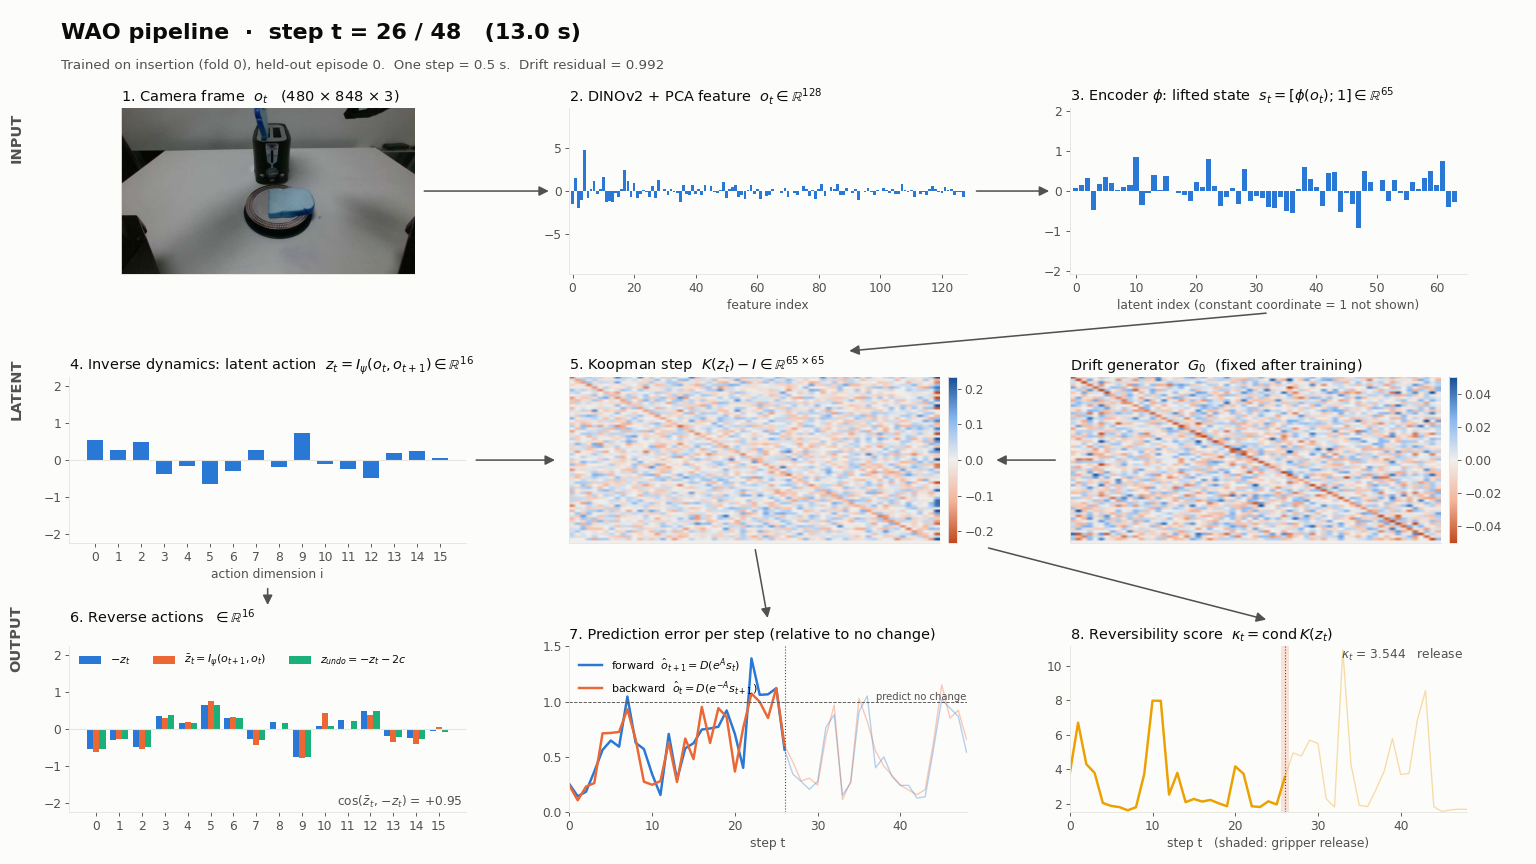
\includegraphics[width=0.8\textwidth]{figs/fig_walkthrough.png}
	\caption{All {\method} variables at step 26 of a held-out insertion episode (13.0\,s, the first release): camera frame, feature $o_t$, lifted state $s_t$, latent action $z_t$, step operator $K(z_t)-I$, drift $G_0$, reverse actions, prediction errors and the reversibility score $\kappa_t$. A video of all 49 steps accompanies the paper.}
	\label{f:walk}
\end{figure*}

Fig.~\ref{f:walk} shows every variable of a model trained on insertion (fold 0), on a held-out insertion episode; its labels follow the submitted version and call the drift-equivalent correction an undo of the drop, which Remark~\ref{r:eps} qualifies.
Reversal consistency is strong: the IDM output on the swapped pair nearly mirrors $-z_t$ (cosine $+0.95$ at the release step).
Because the drift residual is 0.992 for this model, $\zundo$ is almost identical to $-z_t$, in line with Proposition~\ref{p:undo}(c).
In this episode $\kappa_t$ does not peak at the release itself (step 26, $\kappa_t=3.5$); its largest values occur at steps 10, 33 and 43, likely other contact events.
The AUROC of Table~\ref{t:main} is an aggregate over many episodes, and single episodes can be noisier.

% =====================================================================
\section{Controlled Studies with Known Drift} \label{a:toy}

Section~\ref{s:toy} reports the study with dissipative drift and ground-truth reversibility (\texttt{code/toy\_reversibility.py}; per-run results in \texttt{results/toy\_runs/}).
On a single CPU core each Koopman run takes about three minutes and each MLP run about one and a half.
This appendix keeps the earlier study with constant drift (\texttt{code/toy\_bik\_lam.py}), in which every step can be undone.

\begin{table}
	\centering
	\caption{Two-dimensional point with constant drift $g$, observed through a random nonlinear lift. The analytic undo action is $u'=-u-2g$. Return error is the simulator distance to $p_t$ after executing the undo action, divided by the step length.}
	\label{t:toy}
	\footnotesize
	\setlength{\tabcolsep}{4pt}
	\begin{tabular}{lcc}
		\toprule
		Quantity & No reversal loss & Reversal loss \\
		\midrule
		Forward relative error & 0.023 & 0.013 \\
		Backward relative error (never trained) & 0.012 & 0.009 \\
		$\cos(\text{IDM}(o_{t+1},o_t),-z)$ & 0.62 & 0.995 \\
		No-op code size $\|z_{\text{no-op}}\|/\mathrm{rms}(z)$ & 0.36 & 0.48 \\
		Linear probe $R^2$, $z\to u$ & 0.84 & 0.89 \\
		Return error, model undo action & 0.34 & 0.26 \\
		Return error, naive $u'=-u$ & 1.15 & 1.15 \\
		Mean $|u_{\text{undo}}-(-u-2g)|$ (naive: 0.5) & 0.19 & 0.15 \\
		\bottomrule
	\end{tabular}
\end{table}

To test the theory where the ground truth is known, we simulate a two-dimensional point $p_{t+1}=p_t+\Delta t\,(g+u)$ with constant drift $g=(0,-0.5)$, actions $u\in[-1,1]^2$ and $\Delta t=0.1$, observed only through a fixed random two-layer $\tanh$ lift to 32 dimensions.
A Koopman model with $d=8$, $m=2$ and a constant coordinate is trained for 6,000 steps on forward transitions only, once without and once with the reversal-consistency loss (Table~\ref{t:toy}).
Errors are relative to predicting no change and evaluated on 8,000 fresh transitions.
\begin{itemize}
	\item Backward prediction through the exact inverse is as accurate as forward prediction although it is never trained, as Proposition~\ref{p:inverse} predicts.
	\item The IDM is not reversal-consistent by itself (cosine 0.62); the reversal loss makes it so (0.995) and, without an anchor, moves part of the drift into the latent code (no-op code size 0.48), as Proposition~\ref{p:gauge} allows.
	\item The undo action is found by planning in the model, mapped to real actions with a linear probe fitted on labeled transitions (which fixes the gauge), and executed in the simulator. It returns the point to within 0.26--0.34 step lengths, whereas naively negating the action misses by 1.15, and the recovered action is close to the analytic $-u-2g$. The remaining error tracks the probe $R^2$ of 0.84--0.89.
\end{itemize}

% =====================================================================
\section{Development Runs} \label{a:dev}

The runs in this appendix were made while designing the evaluation, on insertion, fold 0, with one run per setting.
They are not cross-validated and are reported for completeness.
Where marked, the reversibility AUROC used an earlier release rule that counted gripper openings without a prior hold; that rule fired 3--5 times per episode and was replaced by the rule in Section~\ref{s:setup}, so those AUROC values are not comparable with Table~\ref{t:main}.

\begin{table*}
	\centering
	\caption{Development runs (insertion, fold 0, one run each). Errors are relative to predicting no change. $^\dagger$AUROC with the earlier release rule (not comparable with Table~\ref{t:main}).}
	\label{t:dev}
	\footnotesize
	\setlength{\tabcolsep}{4pt}
	\begin{tabular}{llcccccc}
		\toprule
		Setting & Model & Forward err. & Backward err. & End dist. & Action align. & Joint probe & AUROC \\
		\midrule
		\multirow{4}{*}{Step 0.1\,s} & Sign-rev. LAM & 0.508 & 0.512 & $7.5\times10^5$ & 0.063 & 0.981 & 0.379$^\dagger$ \\
		& {\method} w/o anchor & 0.525 & 0.525 & 1.033 & 0.058 & 0.975 & 0.460$^\dagger$ \\
		& {\method} & 0.538 & 0.540 & 0.981 & 0.056 & 0.982 & 0.426$^\dagger$ \\
		& Two-dir. ref. & 0.521 & 0.522 & 0.851 & 0.032 & 1.048 & 0.436$^\dagger$ \\
		\midrule
		\multirow{4}{*}{Step 0.5\,s} & Sign-rev. LAM & 0.227 & 0.231 & 1.477 & 0.140 & 1.010 & 0.370$^\dagger$ \\
		& {\method} w/o anchor & 0.230 & 0.235 & 0.959 & 0.116 & 1.051 & 0.482$^\dagger$ \\
		& {\method} & 0.235 & 0.241 & 1.049 & 0.137 & 1.047 & 0.472$^\dagger$ \\
		& Two-dir. ref. & 0.232 & 0.233 & 0.734 & 0.086 & 1.280 & 0.473$^\dagger$ \\
		\midrule
		\multirow{3}{*}{\shortstack[l]{Step 0.5\,s,\\new release rule}} & LAM & 0.231 & 0.232 & 0.684 & 0.208 & 1.147 & 0.580 \\
		& {\method}, $\lambda_v=10^{-5}$ & 0.239 & 0.243 & 1.345 & 0.117 & 1.047 & 0.711 \\
		& {\method}, $\lambda_v=0$ & 0.239 & 0.244 & 1.389 & 0.117 & 1.046 & 0.711 \\
		\bottomrule
	\end{tabular}
\end{table*}

\paragraph{Step size.}
A step of 0.1\,s left forward error at about 0.5 of the no-change baseline for every model, because consecutive frames barely differ, and the sign-reversal LAM's rollout diverged by five orders of magnitude (Table~\ref{t:dev}).
A step of 0.5\,s, trained on all five phase offsets, halved the error, and we use it throughout.

\paragraph{Symmetric action blocks.}
Weakening the penalty on the symmetric action blocks ($\lambda_v=10^{-5}$ or 0) left every metric and the drift residual (0.992) essentially unchanged.
The residual therefore does not come from the penalty, which led us to fit $c$ on visited states; Remark~\ref{r:eps} gives the reason it stays near 1.

\paragraph{Fitting the drift-equivalent action.}
Fitting $c$ on whole matrices, $\min_c\|G_0-\sum_ic_iG_i\|_F$, gave a residual of 0.991 on this fold; fitting on visited states, Eq.~(\ref{e:undo}), gives $0.988\pm0.005$ across folds.
Both are near 1 because 16 action generators cannot cancel the drift's effect in a 65-D lifted space.

\paragraph{Release labels.}
With a hold requirement of 1\,s before a gripper opening past 0.9, exactly two releases are found in 41 of 50 insertion and 49 of 50 removal episodes, matching the two slices per episode.
Without the hold requirement, most episodes showed 3--5 spurious releases, because the gripper passes through the holding range while opening and closing.

\paragraph{Feature check.}
To rule out the visual representation as the cause of transfer limits, we trained a linear probe (logistic regression on 256 PCA dimensions, 5-fold episode split) to decode the three scene stages from 40 episodes at 2\,Hz, using the release-based stage labels.
Table~\ref{t:feat} shows that every variant decodes the stage almost perfectly, so we keep the top-camera CLS token with a $2\times4$ grid.

\begin{table}
	\centering
	\caption{Stage decoding from features, balanced accuracy over 5 episode folds (chance 0.333).}
	\label{t:feat}
	\footnotesize
	\begin{tabular}{lc}
		\toprule
		Features & Balanced accuracy \\
		\midrule
		Top camera, CLS + $2\times4$ grid (used) & 0.975$\pm$0.003 \\
		Top camera, CLS + $4\times7$ grid & 0.979$\pm$0.002 \\
		Wrist cameras, CLS + $2\times4$ grid & 0.982$\pm$0.009 \\
		Top $4\times7$ + wrists & 0.984$\pm$0.003 \\
		\bottomrule
	\end{tabular}
\end{table}

% =====================================================================
\section{Implementation Details} \label{a:impl}

\begin{figure}[t]
	\centering
	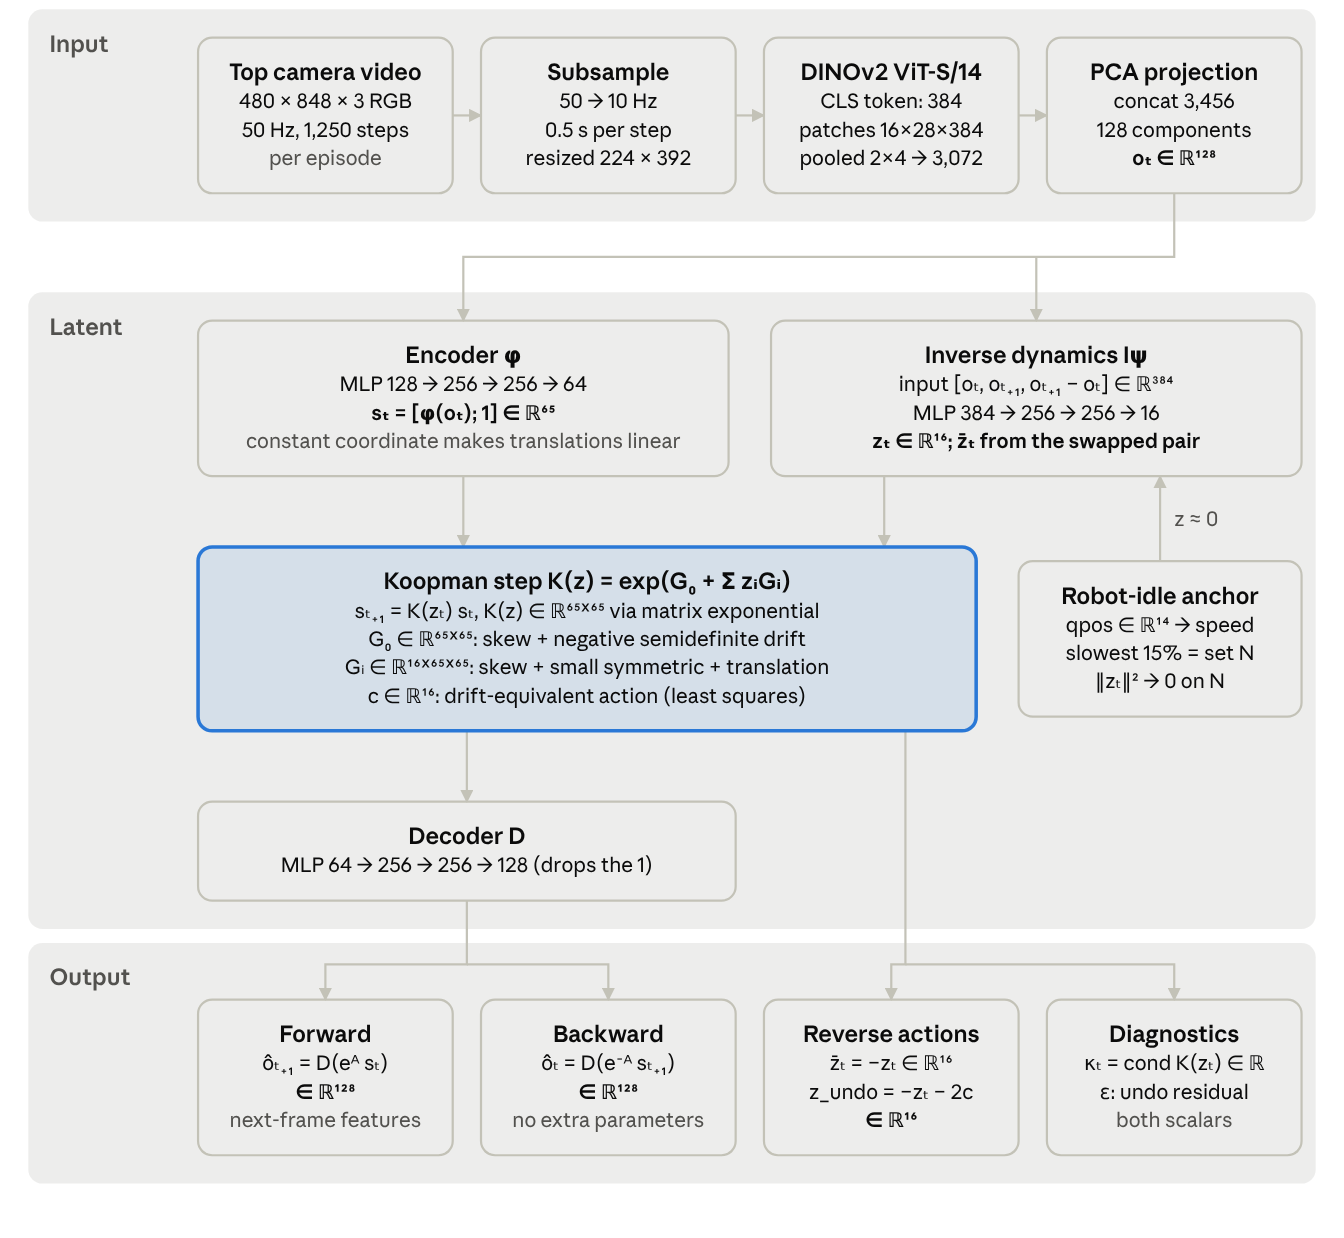
\includegraphics[width=0.7\columnwidth]{figs/fig_pipeline.png}
	\caption{Experimental configuration of {\method} with tensor sizes for the ALOHA toaster data. Each camera image ($480\times848$) is reduced to a feature $o_t\in\R^{128}$, lifted to $s_t\in\R^{65}$ and paired with a latent action $z_t\in\R^{16}$; the forward step, the backward step and both reverse actions all come from one operator $K(z_t)\in\R^{65\times65}$.}
	\label{f:pipeline}
\end{figure}

Fig.~\ref{f:pipeline} shows how Fig.~\ref{f:concept} is instantiated on the ALOHA toaster data.

All models share the following settings.
\begin{itemize}
	\item \textbf{Input:} top camera, $480\times848$, resized to $224\times392$; frozen DINOv2 ViT-S/14; CLS token (384) and a $2\times4$ pooled patch grid (3,072), standardised and reduced by PCA to 128 dimensions with unit average variance.
	\item \textbf{Networks:} head $\phi$ and decoder are MLPs with two hidden layers of 256 units and GELU; the IDM is an MLP on $[o_t,o_{t+1},o_{t+1}-o_t]$ (384 inputs, 16 outputs).
	\item \textbf{Latents:} $d=64$ plus the constant coordinate; $m=16$, with Gaussian noise of 0.05 on $z$ during training.
	\item \textbf{Data:} one step is 0.5\,s (5 frames at 10\,Hz), using all 5 phase offsets for training; the anchor set is the slowest 15\% of steps by joint speed.
	\item \textbf{Optimisation:} Adam, learning rate $10^{-3}$, batch 512, 4,000 steps, gradients clipped at norm 1; $\lambda_b=\lambda_r=\lambda_a=1$, $\lambda_v=10^{-3}$, and $\mathcal{L}_{\mathrm{rec}}$ also includes $10^{-3}\|z_t\|^2$; $c$ is fitted on 2,000 training latents; few-shot adaptation uses 500 IDM steps with batch 256.
	\item \textbf{Evaluation:} the end-distance ratio, stage reach and action alignment pair each test recording of the opposite task with a held-out recording of the training task; distances are measured between decoded features. The two-direction reference rolls out the IDM's actions on the test recording itself. State-specific undo runs 200 Adam steps (learning rate 0.05) on Eq.~(\ref{e:undoss}); the three-step plan starts from the one-step solution followed by two zero actions. All revision-1 diagnostics are computed after the original metrics, with a separate random generator, so the original keys are reproduced exactly (\texttt{code/extras.py}).
	\item \textbf{Compute:} one A100 80\,GB GPU, about 10 minutes per run.
\end{itemize}
LAM baselines use MLP forward and backward models with the same hidden sizes; their reversibility score is the condition number of the forward-model Jacobian with respect to the lifted state.
The 50 cross-validation runs were scheduled two to three at a time to respect the GPU quota of the shared server.
Code, per-fold results and the walkthrough video are released with the paper.


\end{document}
